\documentclass{ieeeaccess}
\usepackage{cite}
\usepackage{amsmath,amssymb,amsfonts}
\usepackage{graphicx}
\usepackage{textcomp}
\usepackage{array}
\usepackage{multirow}
\usepackage{booktabs}
\usepackage{float}
\usepackage{url}
\usepackage[htt]{hyphenat}
\graphicspath{{figures/}{./}}
\tolerance=1000
\emergencystretch=1.5em

\usepackage{bm}
\makeatletter
\AtBeginDocument{\DeclareMathVersion{bold}
\SetSymbolFont{operators}{bold}{T1}{times}{b}{n}
\SetSymbolFont{NewLetters}{bold}{T1}{times}{b}{it}
\SetMathAlphabet{\mathrm}{bold}{T1}{times}{b}{n}
\SetMathAlphabet{\mathit}{bold}{T1}{times}{b}{it}
\SetMathAlphabet{\mathbf}{bold}{T1}{times}{b}{n}
\SetMathAlphabet{\mathtt}{bold}{OT1}{pcr}{b}{n}
\SetSymbolFont{symbols}{bold}{OMS}{cmsy}{b}{n}
\renewcommand\boldmath{\@nomath\boldmath\mathversion{bold}}}
\makeatother

\def\BibTeX{{\rm B\kern-.05em{\sc i\kern-.025em b}\kern-.08em
    T\kern-.1667em\lower.7ex\hbox{E}\kern-.125emX}}

%Your document starts from here ___________________________________________________
\begin{document}
\history{Date of publication xxxx 00, 0000, date of current version xxxx 00, 0000.}
\doi{10.1109/ACCESS.2024.0429000}

\title{Project Garuda: A Privacy-First Edge-AI Home Security\\System on Raspberry Pi~5 with Hailo-8L NPU}
\author{\uppercase{Veeramanikanta Gonugondla}\authorrefmark{1}}

\address[1]{Department of Electronics and Communication Engineering (e-mail: manikantagonugondla@gmail.com)}
\tfootnote{This work was carried out as an independent project. All hardware, software, and cloud services were self-funded.}

\markboth
{Gonugondla: Project Garuda}
{Gonugondla: Project Garuda}

\corresp{Corresponding author: Veeramanikanta Gonugondla (e-mail: manikantagonugondla@gmail.com).}


\begin{abstract}
Nowadays, Home Security Systems are very expensive and depend heavily on the cloud to run AI models. Cloud Dependency involves increased expenses for infrastructure and is also privacy-invasive. We can also opt for open-source alternatives, which come with a trade-off in the integration between hardware and software due to compatibility of various hardware and software libraries. Most DIY setups either detect only motion with no second intelligence check or require a full server rack to run meaningful AI models. No widely available solution integrates real-time edge AI, remote access, voice control, and encrypted data handling on consumer hardware at a meaningful price point and with meaningful integration.
Project Garuda is an attempt to close that gap.
It is an AI-powered home security system built on a Raspberry Pi 5 integrated with a Hailo-8L neural processing unit — a 13 TOPS dedicated AI accelerator that handles deep learning inference without taxing the CPU. The system runs YOLOv8s object detection through a GStreamer pipeline managed by Hailo's TAPPAS framework, silently logging person detections and triggering alerts when it identifies dangerous objects — knives, scissors, or hammers — in frame. Alerts are dispatched as OTP-authenticated emails with a 60-second cooldown to prevent spam.
The backend is a FastAPI web server, accessible remotely through a Cloudflare tunnel at api.veeramanikanta.in, secured with PBKDF2-SHA256 session authentication, a master key system, per-endpoint rate limiting, and strict CORS and security header policies. The frontend is a Progressive Web App. Video clips can be recorded, AES-256 encrypted, and sent over SSH to a remote host. Live video is available over both WebRTC and MJPEG. A voice assistant named Narada runs as a background thread, responding to a configurable wake word and routing commands either through rule-based matching or a Groq-hosted LLM — the same model backing the web UI's streaming chat interface.
The system supports six operating modes — Do Not Disturb, email-off, idle, night, emergency, and privacy — schedulable automatically or set manually. Supporting subsystems include ARP-based LAN device presence tracking, a 180-second deadman watchdog that fires a tamper alert on missed heartbeats, a SQLite-backed offline event sync queue, and a multi-tier logging pipeline with rotation across persistent text and JSON files.
The goal is a self-hosted, privacy-first security system that thinks at the edge, costs under US\$450--500 to build, and doesn't phone home to anyone.
\end{abstract}

\begin{keywords}
Edge AI, GStreamer, Hailo-8L, home security, neural processing unit, object detection, privacy, Raspberry Pi, real-time inference, YOLOv8.
\end{keywords}

\titlepgskip=-21pt

\maketitle

\section{Introduction}
\label{sec:introduction}
\PARstart{H}{ome} security systems have evolved from passive alarm triggers to intelligent platforms that can recognise specific objects, persons, and behaviours in real time. However, the commercial market remains bifurcated. On one end, cloud-dependent solutions from established vendors offload inference to remote data centres, introducing recurring subscription costs, network-latency penalties, and privacy concerns because raw video leaves the premises~\cite{b1}. On the other end, do-it-yourself (DIY) setups based on single-board computers typically offer motion detection at best, with no second-stage intelligence check and no integrated alert, voice, or encrypted-evidence pipeline~\cite{b2}.

Recent advances in dedicated neural processing units (NPUs) have begun to close this gap by bringing deep-learning inference to the edge at watt-level power budgets. The Hailo-8L, for example, delivers 13~TOPS of INT8 compute over a single PCIe Gen3 lane and can be attached to a Raspberry Pi~5 through a standard M.2 HAT, giving a sub-US\$500 platform enough throughput to run YOLOv8-class detectors at more than 50~FPS without taxing the host CPU~\cite{b3}. Bueno \emph{et~al.}~\cite{b4} recently validated this exact hardware combination for real-time YOLOv8 inference in microscopy, confirming that the RPi~5 plus Hailo-8L pipeline can match GPU-accelerated systems in accuracy while consuming a fraction of the power.

\subsection{Related Work}
Edge-deployed YOLO variants have been explored across several domains. Xu \emph{et~al.}~\cite{b1} proposed FL-YOLO, a depthwise-separable variant running on an NVIDIA Jetson TX1 inside a coal-mine surveillance system, achieving 36.7~FPS at 76.7\% AP through an edge-cloud cooperation framework. Al~Amin \emph{et~al.}~\cite{b5} implemented YOLOv3~Tiny on a Xilinx Kria KV260 FPGA, reaching 15~FPS at 99\% accuracy for traffic-light classification at 3.5~W --- demonstrating that dedicated accelerators can outperform general-purpose GPUs in power efficiency for fixed inference tasks. Dong \emph{et~al.}~\cite{b6} introduced PG-YOLO, which replaces standard convolutions in YOLOv5s with Ghost modules and applies channel pruning plus knowledge distillation to achieve a $9\times$ compression with only 0.1\% accuracy loss, a technique directly applicable to NPU deployment. Chung \emph{et~al.}~\cite{b7} proposed YOLO-LSD with CBAM attention for detecting small pedestrians at long range, and Cheng~\cite{b8} presented RMN-YOLO with multi-scale edge enhancement for defect detection, both contributing architectural ideas for improving small-object recall on resource-constrained hardware. The Ultralytics YOLOv8 framework~\cite{b9} provides the baseline architecture and training pipeline used in this work, and the Hailo TAPPAS framework~\cite{b10} supplies the GStreamer elements that dispatch inference to the NPU.

Despite this body of work, no published system integrates all of the following on a single consumer-grade edge device: real-time multi-class object detection with a dedicated NPU, a cascaded classifier and depth-based anti-spoof stage, encrypted evidence capture, a voice assistant with LLM fallback, ARP-based presence monitoring, a tamper-detection watchdog, and a remotely accessible web server with session authentication and OTP two-factor verification.

\subsection{Contributions}
This paper presents Project Garuda, an end-to-end AI home security system that runs entirely on a Raspberry Pi~5 with a Hailo-8L AI HAT+. The principal contributions are:

\begin{enumerate}
\item A custom-fine-tuned YOLOv8s detector for four security-relevant classes (Hammer, Knife, Person, Scissors) trained on a 4{,}982-image dataset and compiled to an INT8 HEF, achieving a test mAP{@}0.5 of 0.847 at 52.22~FPS on the Hailo-8L.
\item A three-stage cascade architecture (YOLOv8s + MobileNetV2 classifier + MiDaS depth estimator) that adds weapon verification and photo/screen spoof rejection with less than 5~ms additional latency.
\item A twelve-engine software architecture --- detection, alert, voice assistant, mode controller, presence monitor, web server, authentication, deadman watchdog, logging, and more --- integrated under a single FastAPI application and exposed through a Cloudflare tunnel, delivering a complete security platform with no cloud inference dependency.
\item A comprehensive evaluation covering training convergence, per-class metrics, confusion structure, hardware throughput, and a dataset-scaling study from 359 to 4{,}982 training images.
\end{enumerate}

\subsection{Paper Organisation}
The remainder of this paper is organised as follows. Section~\ref{sec:methodology} describes the methodology, covering every engine from hardware through logging. Section~\ref{sec:flowchart} presents the system flowchart and block diagram. Section~\ref{sec:specs} consolidates hardware, software, model, and dataset specifications. Section~\ref{sec:results} reports training and inference results. Section~\ref{sec:conclusion} concludes with a summary of findings and directions for future work.

\section{Methodology}
\label{sec:methodology}
Project Garuda is implemented as a collection of loosely coupled engines that share state through a mode controller and a multi-tier logging layer. This section describes every engine in turn---hardware, the GStreamer inference pipeline, the detection callback and the optional cascade, alerting, the voice assistant, mode control, LAN presence, the web server, authentication, the deadman watchdog, and the logging subsystem. Each engine is introduced with a short functional overview, followed by its implementation details, supporting tables, and its control-flow diagram.

\subsection{Hardware Engine}
The hardware engine hosts all other subsystems on a single consumer board and offloads inference to a dedicated neural accelerator so that the general-purpose CPU remains free for the web server, voice pipeline, and logging. This is the key architectural decision that lets the system run real-time object detection, fine-grained classification, and monocular depth on the edge without thermal throttling.

The host board is a Raspberry Pi 5 running a Broadcom BCM2712 quad-core Cortex-A76 at 2.4~GHz with 8~GB LPDDR4X memory on 64-bit Raspberry Pi OS. A Hailo-8L AI HAT+ is attached through a PCIe Gen3 $\times$1 M.2 M-Key interface and is exposed to the operating system as \texttt{/dev/hailo0}. The HailoRT driver is installed as a DKMS kernel module (\texttt{hailo\_pci}) so that the device survives kernel upgrades, and the TAPPAS 3.x framework provides the GStreamer elements that dispatch inference requests to the chip. The Hailo-8L itself delivers 13~TOPS of INT8 neural compute and runs all three models of the cascade---the YOLOv8s detector, the MobileNetV2 classifier, and the MiDaS Small depth estimator---asynchronously with no CPU involvement during the forward pass. Video is sourced either from a USB webcam captured through V4L2 (GStreamer \texttt{v4l2src} on \texttt{/dev/video0}) or from a Sony IMX708 Camera Module v3 connected through the CSI-2 MIPI interface (GStreamer \texttt{libcamerasrc} via \texttt{libcamera}). The Pi's Gigabit Ethernet or 802.11ac Wi-Fi interface serves two roles: outbound HTTPS through the Cloudflare tunnel for remote access, and ARP traffic on the local subnet for device-presence scanning. Model files (\texttt{.hef}), the operating system, and all persistent logs live either on the microSD card or on an external USB-3 SSD. The hardware topology is illustrated in Fig.~\ref{fig:hw_layer}.

\begin{figure}[!t]
\centering
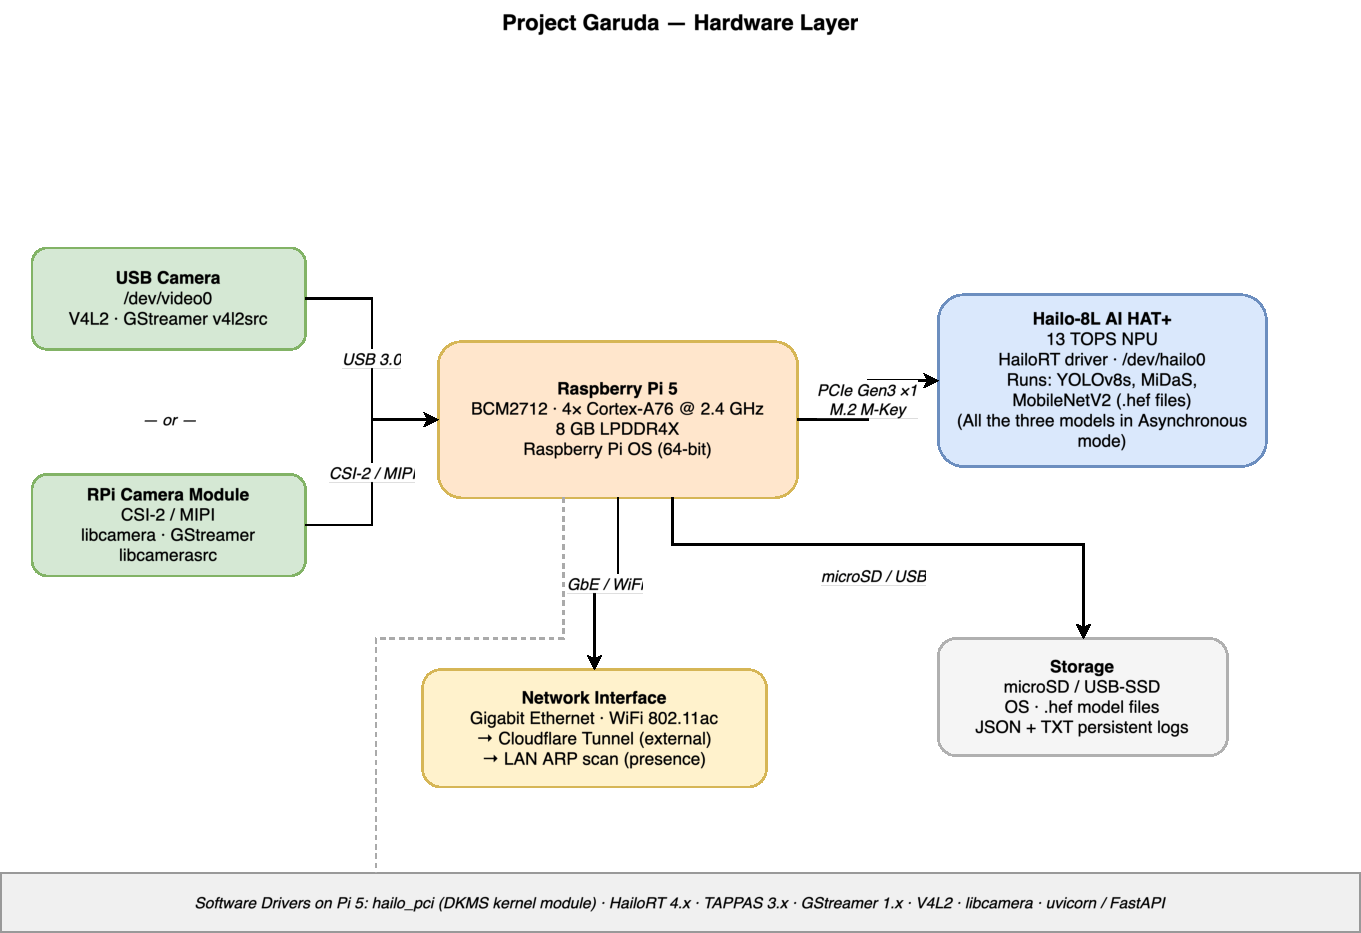
\includegraphics[width=\columnwidth]{garuda_hardware_layer.drawio.pdf}
\caption{Hardware engine: Raspberry Pi 5 host with the Hailo-8L AI HAT+ attached over PCIe Gen3 $\times$1, CSI-2/USB camera input, and Gigabit Ethernet / Wi-Fi uplink.}
\label{fig:hw_layer}
\end{figure}

\subsection{GStreamer TAPPAS Pipeline Engine}
The GStreamer engine is the video ingestion and inference core. It captures raw frames, runs them through the Hailo accelerator, and produces time-aligned annotated buffers that downstream engines can subscribe to.

The pipeline is built in the \texttt{GStreamerDetectionApp} class (\texttt{Garuda\_web.py}) which extends the base \texttt{GStreamerApp} from \texttt{hailo\_rpi\_common.py}. It accepts three video source element types---\texttt{v4l2src} for USB cameras, \texttt{libcamerasrc} for the Raspberry Pi CSI-2 camera, and \texttt{filesrc} for recorded video---and normalises every source through \texttt{videoscale} and \texttt{videoconvert} elements so that the inference branch always receives frames at the network's native resolution and pixel format. From the preprocessor the pipeline forks into two parallel branches. The inference branch routes frames into \texttt{HailoNet}, the GStreamer element that dispatches inference requests over PCIe to the Hailo-8L, and then into a \texttt{HailoFilter} element that runs non-maximum suppression (NMS) on the raw network tensor output (IoU threshold $\leq 0.45$, confidence threshold $\geq 0.35$). In parallel, a bypass queue carries the time-aligned raw frames forward. Both branches converge at the \texttt{HailoMuxer}, which synchronises the annotated inference results with the corresponding raw frame before pushing the merged buffer to an \texttt{identity} element where the \texttt{app\_callback} user probe is attached. After the callback, a \texttt{HailoOverlay} element renders bounding boxes and class labels onto the frame, and the final buffer is delivered to either a display sink or a video sink depending on runtime configuration. The complete pipeline topology is shown in Fig.~\ref{fig:gstreamer}.

\begin{figure}[!t]
\centering
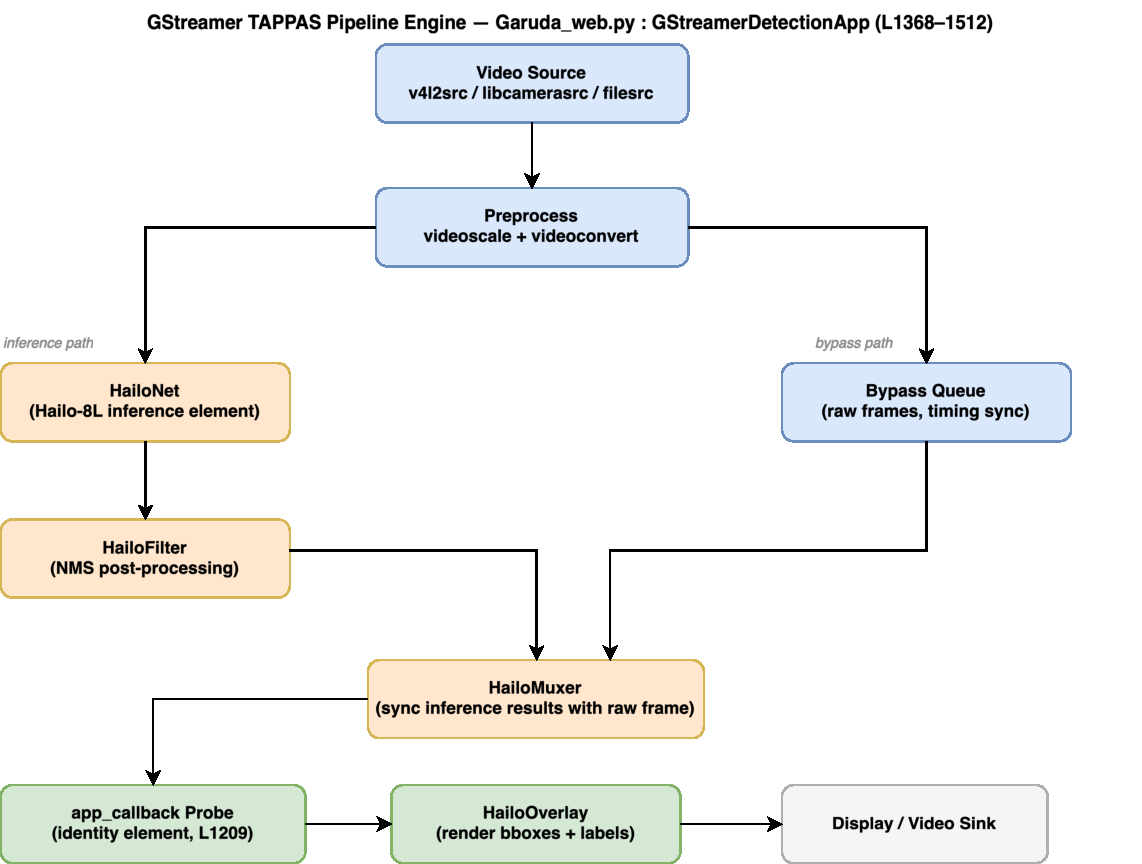
\includegraphics[width=\columnwidth]{garuda_gstreamer_engine.drawio-2.pdf}
\caption{GStreamer TAPPAS pipeline: source $\to$ preprocess $\to$ (HailoNet + NMS $\parallel$ bypass queue) $\to$ HailoMuxer $\to$ identity callback $\to$ overlay $\to$ sink.}
\label{fig:gstreamer}
\end{figure}

\subsubsection{Input Preprocessing}
Before any frame reaches the NPU it is letterbox-resized from the native camera resolution to the network input size of $640\times640$ while preserving aspect ratio, and then normalised to the Hailo-8L's INT8 quantisation range. The letterbox pass pads the shorter axis with grey pixels so that the content is not distorted; the resulting scale factor $s$ and padding offset $(p_x,p_y)$ are retained so that detected bounding boxes can be mapped back to the original frame for overlay rendering and for the alert engine's evidence crops. Formally,
\begin{equation}
s = \min\!\!\left(\frac{640}{W},\;\frac{640}{H}\right)\!,\;
p_x=\frac{640 - sW}{2},\;
p_y=\frac{640 - sH}{2}.
\end{equation}
For a detection expressed as $(x_{\mathrm{net}},y_{\mathrm{net}},w_{\mathrm{net}},h_{\mathrm{net}})$ in the network frame the inverse map
\begin{equation}
x = \frac{x_{\mathrm{net}} - p_x}{s},\quad y = \frac{y_{\mathrm{net}} - p_y}{s}
\end{equation}
recovers coordinates in the original image. Pixel intensities are scaled from $[0,255]$ to the network's INT8 domain during post-training quantisation, so no floating-point preprocessing is required at runtime---the chip accepts the raw YUV-to-RGB converted frame directly.

\subsection{Detection Engine}
The detection engine is the first consumer of inference results. It decides, on every frame, whether the scene contains anything that should be logged, and whether a danger-class detection is reliable enough to fire the alert pipeline.

The engine is implemented as the \texttt{app\_callback} function (\texttt{Garuda\_web.py}) attached as a GStreamer pad probe on the \texttt{identity} element sitting immediately after the \texttt{HailoMuxer}. On every buffer the probe calls \texttt{get\_numpy\_from\_buffer} to obtain a zero-copy NumPy view of the pixels and \texttt{hailo.get\_roi\_from\_buffer} to retrieve the root \texttt{HAILO\_ROI} metadata object. Every \texttt{HAILO\_DETECTION} child is iterated and filtered by a confidence threshold of $0.3$ (\texttt{DETECTION\_THRESHOLD}). Surviving detections are classified by label. Objects matching the \texttt{WATCH\_LABELS} set (\textit{Person} / \textit{person}) are appended to the persistent detection log with a 30-second per-label cooldown so that a long-dwelling subject does not flood the log. Objects matching the \texttt{DANGER\_LABELS} set (\textit{Knife}, \textit{Scissors}, \textit{Hammer}) increment a per-label \texttt{\_label\_consec\_frames} counter; once the counter passes a small threshold (three consecutive frames in the deployed configuration), \texttt{trigger\_software\_alert} is invoked and the full alert pipeline is fired. In parallel, \texttt{\_class\_counts\_today}, \texttt{\_total\_frames}, and \texttt{\_detections\_today} counters are maintained for the dashboard, and the \texttt{user\_app\_callback\_class.set\_frame}/\texttt{get\_frame} interface exposes the current annotated frame to the MJPEG and WebRTC streaming paths. The detection callback flow is depicted in Fig.~\ref{fig:detect}.

\begin{figure}[!t]
\centering
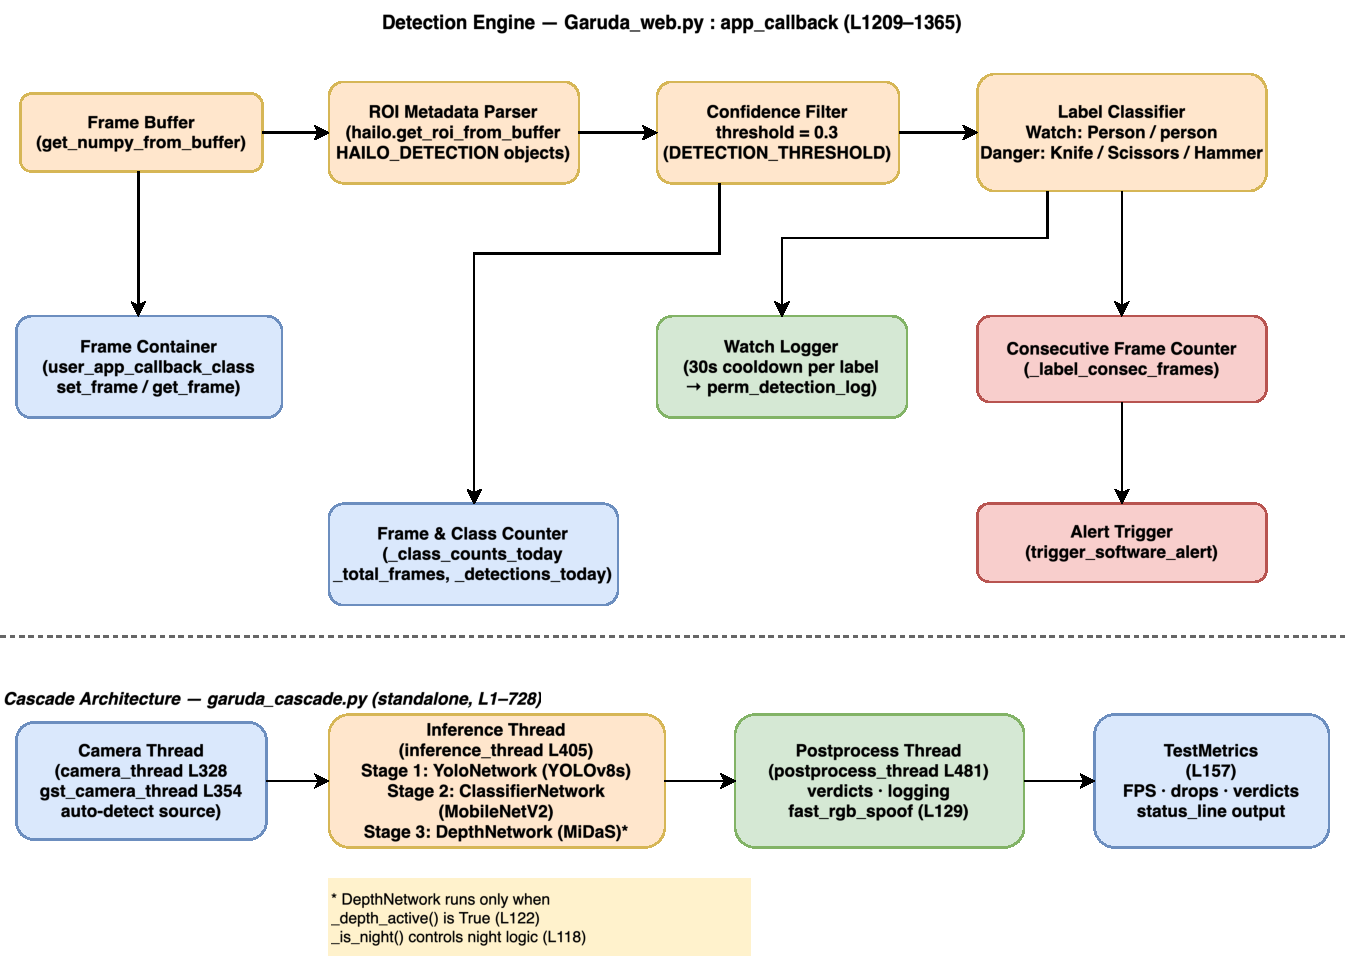
\includegraphics[width=\columnwidth]{garuda_detection_engine.drawio.pdf}
\caption{Detection engine callback: metadata extraction, confidence filter, watch/danger label routing, and consecutive-frame gating before alert dispatch.}
\label{fig:detect}
\end{figure}

\subsection{Cascade Architecture (garuda\_cascade.py)}
A standalone cascade pipeline (\texttt{garuda\_cascade.py}, not invoked by \texttt{Garuda\_web.py}) implements a three-stage inference chain designed for higher-accuracy person verification and photo/screen spoof rejection. A \texttt{camera\_thread} (or \texttt{gst\_camera\_thread}) feeds raw frames into an \texttt{inference\_thread} that runs three models sequentially. Stage 1 uses \texttt{YoloNetwork} (YOLOv8s) to detect persons and objects and return bounding boxes. Stage 2 crops each detected person region and passes it through \texttt{ClassifierNetwork} (MobileNetV2) for fine-grained \textit{Safe} vs \textit{Weapon} classification on the crop. Stage 3 optionally runs \texttt{DepthNetwork} (MiDaS Small) for monocular depth estimation, enabled only when \texttt{\_depth\_active()} returns \texttt{True}---a gate that itself depends on configuration and the \texttt{\_is\_night()} time-of-day check. A \texttt{postprocess\_thread} consumes the per-frame verdicts, applies \texttt{fast\_rgb\_spoof} for a fast liveness variance check, writes final verdicts to disk, and a \texttt{TestMetrics} object tracks per-run FPS, frame drops, and verdict distribution for benchmarking and evaluation. The per-stage latency budget is detailed in Table~\ref{tab:cascade_latency}, and the decision matrix across operating scenarios is given in Table~\ref{tab:cascade_matrix}.

\begin{table}[!t]
\caption{\textbf{Cascade Latency Budget (Hailo-8L, Pi~5)}}
\label{tab:cascade_latency}
\centering
\begin{tabular}{|l|l|}
\hline
\textbf{Component} & \textbf{Measured Value} \\
\hline
T$_{\text{capture}}$ (GStreamer appsink pull) & $\sim$1~ms \\
T$_{\text{YOLO}}$ (NPU, Hailo-8L HW) & 18.38~ms \\
T$_{\text{crop\_preprocess}}$ (NumPy resize) & $\sim$0.5~ms \\
T$_{\text{classifier}}$ (MobileNetV2 @ 500+ FPS) & $<$2~ms \\
T$_{\text{depth}}$ (MiDaS @ 200+ FPS) & $<$5~ms \\
T$_{\text{decision}}$ (NumPy variance) & $<$0.1~ms \\
T$_{\text{alert}}$ (SMTP, async) & $\sim$800~ms \\
T$_{\text{alert}}$ (TTS, async) & $\sim$200~ms \\
T$_{\text{processing}}$ (detection only, end-to-end) & $\sim$22~ms \\
T$_{\text{total}}$ (with async alert) & $\sim$22~ms + async \\
\hline
\end{tabular}
\end{table}

\begin{table*}[!t]
\caption{\textbf{Cascade Decision Matrix Across Operating Scenarios}}
\label{tab:cascade_matrix}
\centering
\small
\begin{tabular}{|p{4.2cm}|p{2.8cm}|p{3cm}|c|c|p{2.5cm}|}
\hline
\textbf{Scenario} & \textbf{Model(s)} & \textbf{mAP{@}0.5} & \textbf{FPS} & \textbf{Latency} & \textbf{Alert Type} \\
\hline
Daytime --- dangerous object & v5 & 0.866--0.967 & 52.22 & 22\,ms & Direct YOLO \\
Daytime --- person + weapon & v5 + MobileNetV2 & 0.647 + 99.6\% cls. & 52.22 & 24\,ms & Cascade \\
Night --- person + anti-spoof & v5 + MiDaS & 0.647 + depth & 52.22 & 27\,ms & Depth-verified \\
Photo/screen spoof & MiDaS & N/A & 52.22 & 27\,ms & Spoof label \\
\hline
\end{tabular}
\end{table*}

\subsection{Alert Engine}
The alert engine converts a confirmed danger detection into a user-visible notification and, when configured, a persistent piece of evidence. Entry is through \texttt{trigger\_software\_alert}, which first acquires \texttt{\_mode\_lock} and short-circuits if \texttt{MODE\_DND} or \texttt{MODE\_IDLE} is active; otherwise it sets \texttt{\_alert\_active} and \texttt{\_alert\_end\_time} to raise a 3-second banner state, then calls \texttt{push\_urgent\_ws} to broadcast a JSON alert payload to every connected WebSocket client so that browsers, the PWA, and the mobile interface update immediately. Concurrently, \texttt{send\_email\_alert} dispatches an SMTP-SSL email to the configured administrator address subject to a 60-second cooldown and the \texttt{MODE\_EMAIL\_OFF} flag, which together prevent alert storms on repeated detections. A separate path handles OTP delivery via \texttt{send\_otp\_via\_email} for admin login and password-reset flows, while \texttt{\_send\_tamper\_email} is reserved for deadman-watchdog violations. When evidence capture is requested, the \texttt{clip\_start} / \texttt{clip\_stop} pair brackets a short video segment around the triggering frame, \texttt{\_encrypt\_clip\_aes256} encrypts the clip using AES-256-CBC with a key drawn from the \texttt{EXFIL\_AES\_KEY} environment variable (never checked into source control), and \texttt{\_ssh\_upload} combined with \texttt{exfiltrate\_clip} transfers the encrypted file over SSH via \texttt{paramiko} to a configurable remote host. Privacy mode is honoured in-line: when active, a Gaussian blur of kernel size $k=51$ and $\sigma=30$ is applied to all person bounding boxes before the MJPEG/WebRTC publisher pushes the frame, so stored clips and remote streams never contain an identifiable subject. The alert flow is summarised in Fig.~\ref{fig:alert}.

\begin{figure}[!t]
\centering
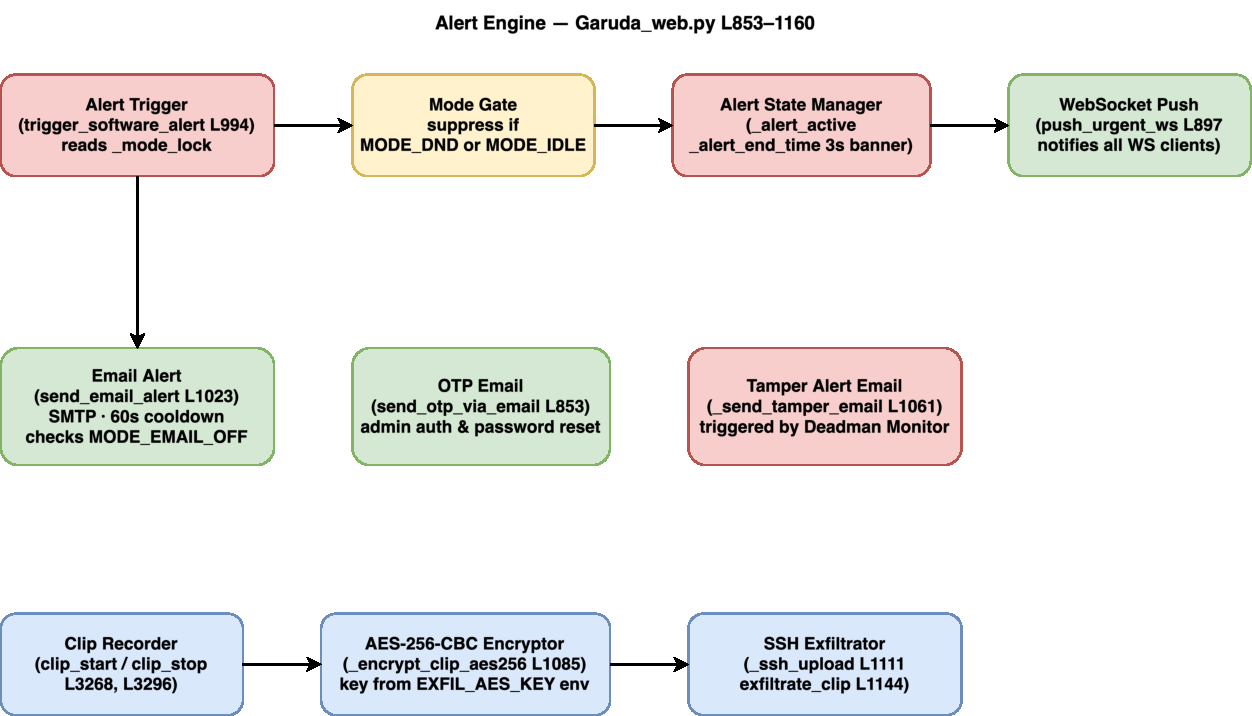
\includegraphics[width=\columnwidth]{garuda_alert_engine.drawio.pdf}
\caption{Alert engine: mode gate, WebSocket broadcast, SMTP email with 60\,s cooldown, AES-256-CBC clip encryption, and SSH exfiltration to a remote host.}
\label{fig:alert}
\end{figure}

\subsection{Voice Assistant Engine (Narada)}
Narada is the spoken interface to Project Garuda. It runs as a background daemon thread that continuously listens on the system microphone through \texttt{speech\_recognition}'s \texttt{sr.Microphone} with automatic energy-threshold adjustment so that changes in ambient noise do not produce false triggers. Every audio frame is first checked against the configurable wake word (\texttt{NARADA\_WAKE\_WORD}, default \texttt{"narada"}); only utterances that follow the wake word are forwarded to the \texttt{sr.Recognizer} for cloud-backed speech-to-text. The transcribed text is handed to \texttt{apply\_rule\_based\_command}, which attempts to match against a set of built-in rules and the user-defined \texttt{CUSTOM\_VOICE\_COMMANDS} registry before returning a match. If no rule matches, the text is forwarded to \texttt{query\_local\_llm}, which calls the Groq API (\texttt{gpt-oss-120b}) for natural-language intent resolution. Groq's response is a structured JSON payload that \texttt{\_apply\_llm\_result} maps to concrete system actions---toggling mode flags, composing emails, or querying system state. Both the rule-based and the LLM-based paths write their input transcripts and output responses to the \texttt{voice\_assistant\_log} and \texttt{voice\_responses} in-memory buffers, which the logging engine periodically flushes to \texttt{perm\_voice\_log.txt}. The voice pipeline is diagrammed in Fig.~\ref{fig:voice}.

\begin{figure}[!t]
\centering
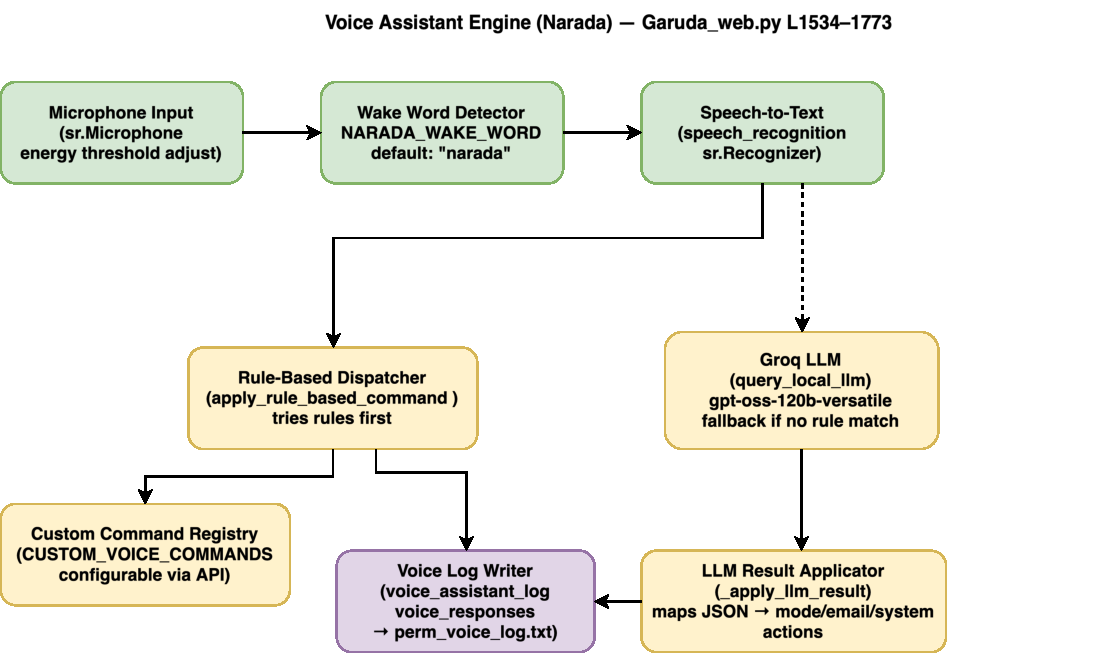
\includegraphics[width=\columnwidth]{garuda_voice_engine.drawio.pdf}
\caption{Voice assistant Narada: microphone capture, wake-word gate, speech-to-text, rule-based dispatcher, and Groq LLM fallback for open-ended intents.}
\label{fig:voice}
\end{figure}

\subsection{Mode Controller}
Six boolean operating flags---\texttt{MODE\_DND}, \texttt{MODE\_EMAIL\_OFF}, \texttt{MODE\_IDLE}, \texttt{MODE\_NIGHT}, \texttt{MODE\_EMERGENCY}, and \texttt{MODE\_PRIVACY} (default \texttt{True})---gate behaviour across every other engine. The alert engine checks DND and Idle before broadcasting; the web server checks Privacy before publishing a stream; the voice engine checks Emergency before acting on potentially destructive commands. All flag reads and writes are serialised through \texttt{\_mode\_lock} (a \texttt{threading.Lock}) to prevent races between the GStreamer callback thread, the schedule daemon, and the web request handlers. User-defined modes beyond the built-in six are stored in the \texttt{CUSTOM\_MODES} registry and can be created or deleted via the configuration API. A \texttt{\_schedule\_monitor} daemon thread wakes every 30~seconds and calls \texttt{\_time\_in\_range} against entries in the \texttt{MODE\_SCHEDULE} dictionary loaded from \texttt{config.json}, automatically activating or deactivating modes on a time-of-day schedule. Runtime changes to any flag---whether from the REST API (\texttt{POST /api/modes}), from the voice assistant, or from the scheduler---are immediately persisted to \texttt{config.json} through \texttt{save\_config} and are restored on the next startup through \texttt{load\_config}. The mode controller architecture is shown in Fig.~\ref{fig:mode}.

\begin{figure}[!t]
\centering
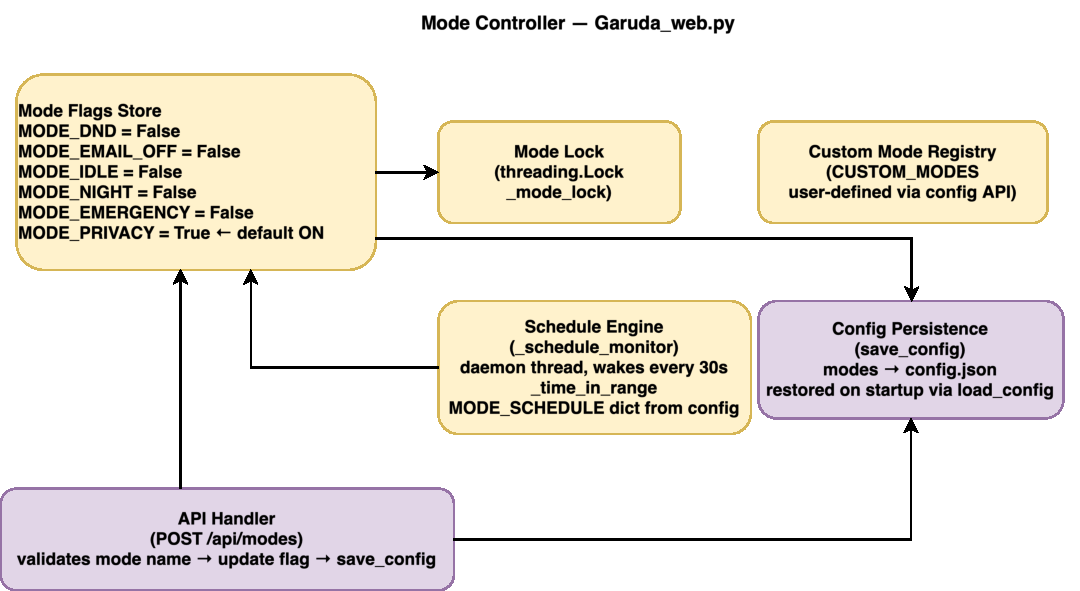
\includegraphics[width=\columnwidth]{garuda_mode_controller.drawio.pdf}
\caption{Mode controller: lock-protected flag store, time-of-day scheduler, and configuration persistence.}
\label{fig:mode}
\end{figure}

\subsection{Presence Monitor}
The presence monitor (\texttt{\_presence\_poller} in \texttt{Garuda\_web.py}) tracks the online/offline status of known LAN devices by running periodic ARP scans directly from the Pi. It issues \texttt{arp\hyp{}scan} or \texttt{ip~neigh} commands through \texttt{subprocess} and parses the returned MAC addresses. The \texttt{KNOWN\_\allowbreak{}DEVICES} dictionary---mapping MAC addresses to human-readable device names---is loaded from \texttt{config.json} at startup and can be updated at runtime through the \texttt{/api/\allowbreak{}devices} REST endpoint followed by \texttt{save\_config}. After each scan the engine compares the discovered MAC set against the previous state stored in \texttt{\_device\_\allowbreak{}presence}; a transition from offline to online, or vice versa, triggers a change event that is immediately pushed to all connected WebSocket clients via \texttt{push\_urgent\_ws}, letting the dashboard update device-status indicators in real time without client polling. The scan interval is tunable (30~s poll with a 90~s grace window in the deployed setup), and unknown MAC addresses are reported to the administrator for registry addition or flagging. The scan loop is illustrated in Fig.~\ref{fig:presence}.

\begin{figure}[!t]
\centering
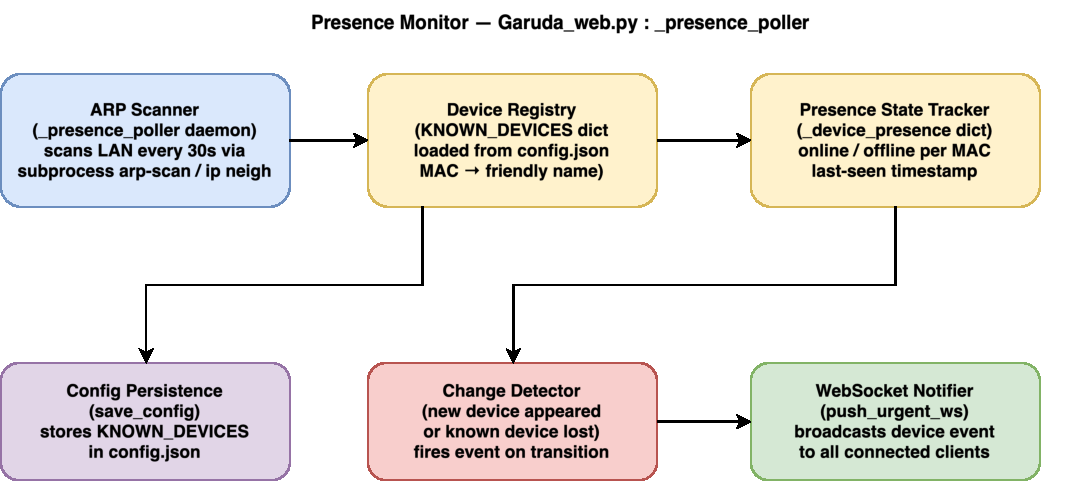
\includegraphics[width=\columnwidth]{garuda_presence_monitor.drawio.pdf}
\caption{Presence monitor: ARP scan loop, known-device comparison, transition-event WebSocket push.}
\label{fig:presence}
\end{figure}

\subsection{Web Server}
The web server (\texttt{run\_web\_app} in \texttt{Garuda\_web.py}) runs a FastAPI application under Uvicorn bound to \texttt{127.0.0.1:\allowbreak{}8080} and is exposed to the public Internet through a Cloudflare tunnel at \texttt{garuda.\allowbreak{}veera\-mani\-kanta.in}; CORS is restricted to \texttt{veera\-mani\-kanta.in}, \texttt{vercel.app}, and \texttt{localhost} origins so that only known frontends can interact with the API. The application defines approximately 45~REST routes organised into functional groups---authentication (\texttt{/login}, \texttt{/logout}, \texttt{/otp}, \texttt{/reset\hyp{}password}, \texttt{/master\hyp{}key}), system state (\texttt{/api/\allowbreak{}state}, \texttt{/api/\allowbreak{}modes}, \texttt{/api/\allowbreak{}config}), logging (\texttt{/api/\allowbreak{}logs/*}, \texttt{/api/\allowbreak{}events} with SQLite-backed catch-up for offline clients), conversational AI (\texttt{/api/\allowbreak{}chat/\allowbreak{}stream} served as Server-Sent Events against the Groq API), device and user management (\texttt{/api/\allowbreak{}devices}, \texttt{/api/\allowbreak{}users}, \texttt{/api/\allowbreak{}feedback}), and media delivery.

Media is served through three parallel channels: an MJPEG endpoint at \texttt{/stream} that pulls the current annotated frame from the \texttt{user\_app\_\allowbreak{}callback\_class} frame buffer, WebSocket endpoints at \texttt{/ws} and \texttt{/ws/\allowbreak{}stream} for real-time alert and frame push, and a WebRTC track (\texttt{Garuda\-Video\-Track}) served via \texttt{aiortc} for low-latency peer connections. Static files for the Progressive Web App frontend are served from the \texttt{garuda\_web/} directory at the root path, giving the browser client a complete interface without any external CDN dependency. The server architecture is depicted in Fig.~\ref{fig:web}.

\begin{figure}[!t]
\centering
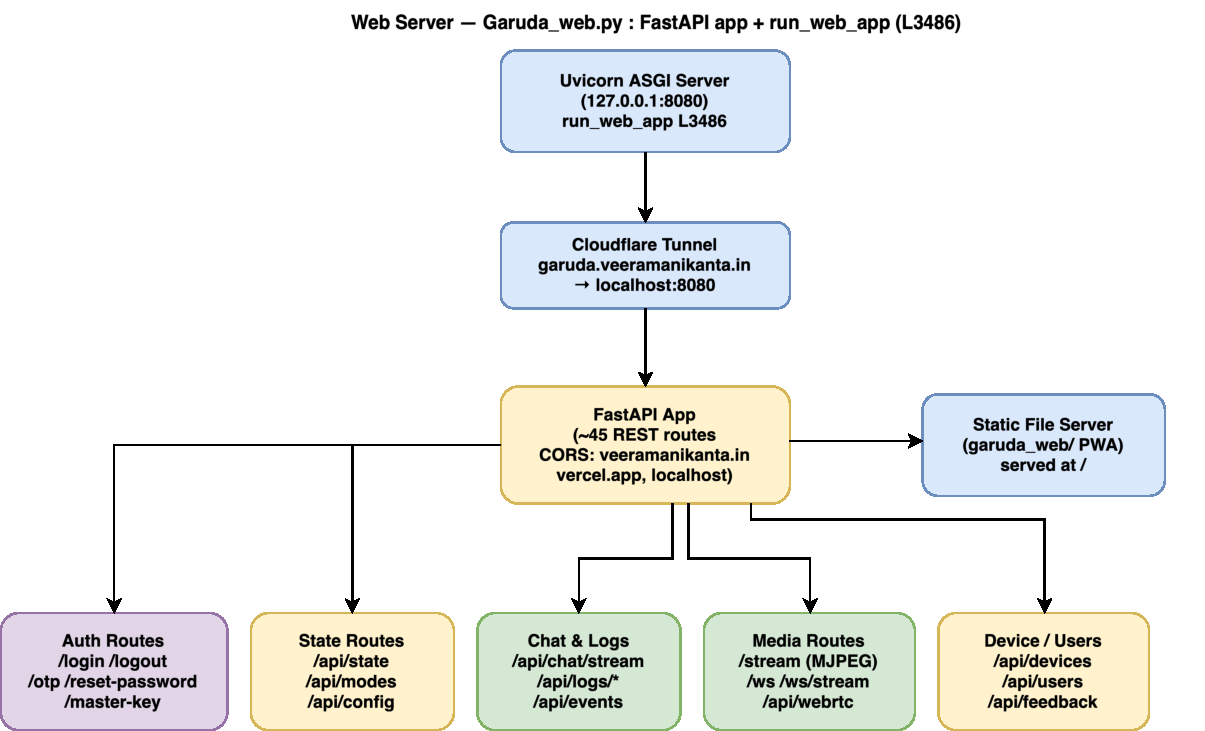
\includegraphics[width=\columnwidth]{garuda_web_server.drawio.pdf}
\caption{Web server: FastAPI under Uvicorn behind a Cloudflare tunnel with $\sim$45 routes and three parallel media channels (MJPEG, WebSocket, WebRTC).}
\label{fig:web}
\end{figure}

\subsection{Auth Engine}
The auth engine handles identity verification and access control for every web API consumer. Passwords are stored as PBKDF2-SHA256 hashes computed with 600{,}000 iterations (\texttt{hashlib.pbkdf2\_hmac}) and unique per-user salts, and are persisted in a JSON user store alongside role labels (\texttt{admin} or \texttt{user}). On a successful login the server generates a cryptographically random session token through \texttt{secrets.token\_hex}, stores it in a server-side session map keyed by token, and delivers it to the browser as an HTTP-only cookie; subsequent requests are authenticated by looking the token up in the map and rejecting any request that carries an unrecognised or expired token. For admin actions that demand a second factor, \texttt{send\_otp\_via\_email} generates a 6-digit code with a 10-minute expiry and delivers it through SMTP; the same mechanism is reused for password-reset flows. A separate Master Key system stores privileged keys in \texttt{master\_keys.json}, independent of the user credential store, so that break-glass operations remain accessible even when normal user accounts are locked or unavailable. Route-level dependency functions enforce role-based access control, granting admin accounts full write access while restricting regular users to read operations and a limited set of state changes. The authentication flow is shown in Fig.~\ref{fig:auth}.

\begin{figure}[!t]
\centering
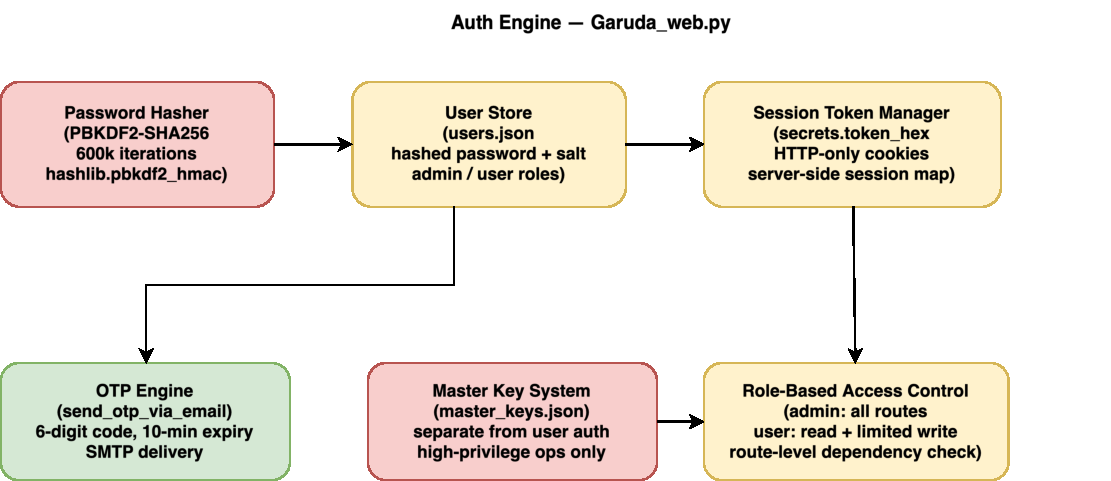
\includegraphics[width=\columnwidth]{garuda_auth_engine.drawio.pdf}
\caption{Auth engine: PBKDF2-SHA256 password store, session-token cookie, OTP 2FA, and separate master-key store.}
\label{fig:auth}
\end{figure}

\subsection{Deadman Monitor}
The deadman monitor (\texttt{\_deadman\_monitor}, \texttt{\_send\_tamper\_email} in \texttt{Garuda\_web.py}) is a tamper-detection watchdog that assumes the absence of regular client heartbeats is evidence of physical interference with the device. Any authenticated browser session sends a periodic ping to \texttt{POST /api/heartbeat}, which updates the \texttt{\_last\_heartbeat} timestamp on the server. The \texttt{\_deadman\_monitor} daemon thread wakes every 10~seconds and computes the elapsed time since the last heartbeat. If the gap exceeds 180~seconds and the system is not in a scheduled maintenance window, the thread treats the condition as a tamper event. On a tamper event two actions execute in parallel: \texttt{trigger\_software\_alert} fires the standard alert pipeline (including the 3-second banner and the WebSocket broadcast to any client that may still be connected), and \texttt{\_send\_tamper\_email} dispatches an SMTP email to the administrator with the event timestamp and the last known system context. The 180-second window is intentionally generous so that it tolerates temporary network drop-outs while still catching the sustained disconnections that indicate the camera or the Pi has been physically moved, covered, or powered down by an intruder. The watchdog logic is diagrammed in Fig.~\ref{fig:deadman}.

\begin{figure}[!t]
\centering
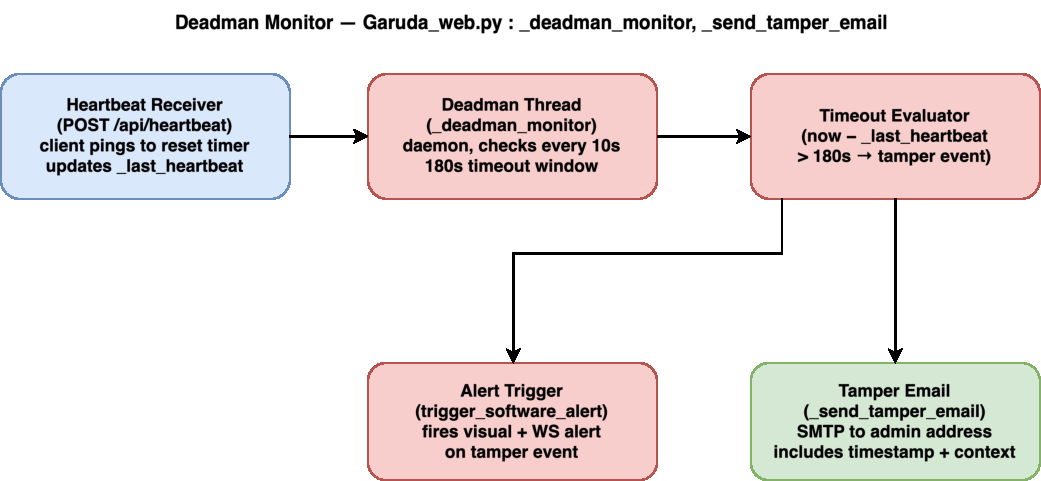
\includegraphics[width=\columnwidth]{garuda_deadman_monitor.drawio.pdf}
\caption{Deadman monitor: 10\,s wake, 180\,s heartbeat deadline, tamper alert + email branch on violation.}
\label{fig:deadman}
\end{figure}

\subsection{Logging Engine}
The logging engine implements a multi-tier persistence strategy designed to balance write performance against durability. All active log streams---alert history, voice command log, system event log, and voice responses---are held in bounded in-memory \texttt{deque}s that accept writes from the GStreamer callback, the voice daemon, the mode controller, and the alert engine without any I/O latency on the write path. A periodic flusher daemon thread drains these deques to disk at a fixed cadence, writing human-readable entries to three permanent append-only text files (\texttt{perm\_detection\_log.txt}, \texttt{perm\_system\_log.txt}, \texttt{perm\_voice\_log.txt}) and updating structured JSON state files (\texttt{alert\_history.json}, \texttt{config.json}) in the \texttt{system\_logs/} directory. A log rotation pass removes entries older than seven days to bound disk growth, running either on the flush cycle or at startup through \texttt{load\_config}. In parallel, every loggable event is also inserted into a SQLite database (\texttt{events.db}) with a microsecond-precision timestamp; the \texttt{/api/events?since=T} endpoint queries this database so that browser clients that were offline for an arbitrary duration can catch up on missed detections, alerts, and state changes without the server having to hold a full event buffer in memory. The logging architecture is shown in Fig.~\ref{fig:logging}.

\begin{figure}[!t]
\centering
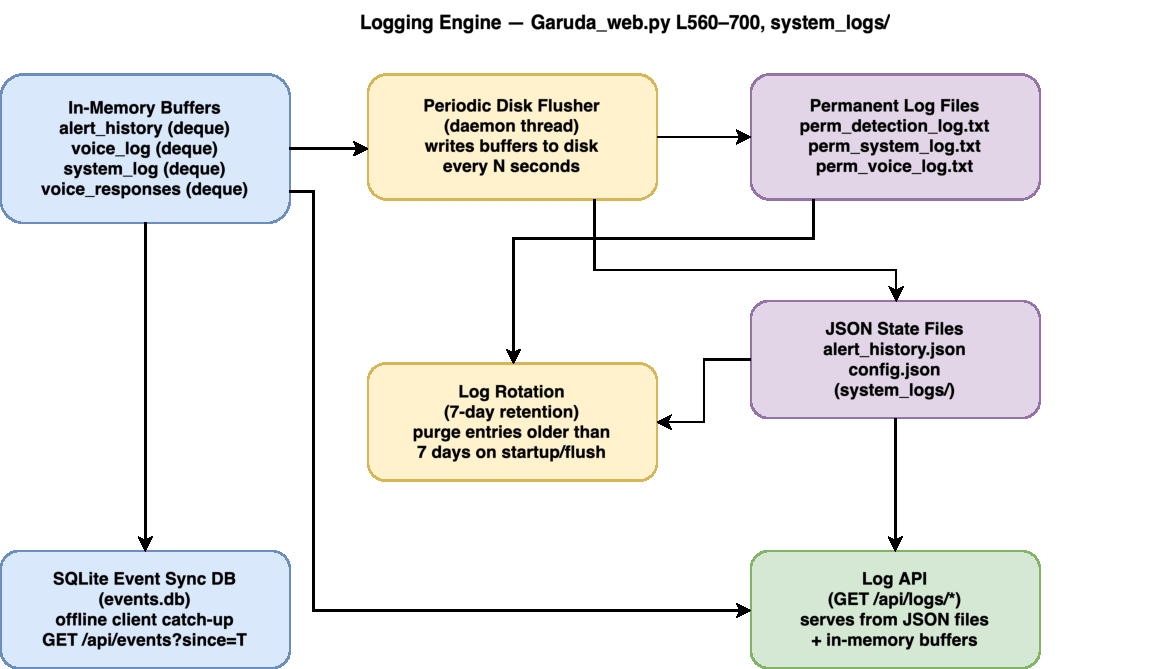
\includegraphics[width=\columnwidth]{garuda_logging_engine.drawio.pdf}
\caption{Logging engine: in-memory deques $\to$ flusher daemon $\to$ permanent text + JSON files + SQLite (\texttt{events.db}) with 7-day rotation.}
\label{fig:logging}
\end{figure}

\section{System Flowchart and Block Diagram}
\label{sec:flowchart}
The end-to-end control flow of Project Garuda is captured in the system flowchart in Fig.~\ref{fig:system_flowchart}, presented as a full-page figure because of its width. The system begins at the Sony IMX708 camera, which delivers frames into the GStreamer TAPPAS pipeline running YOLOv8s object detection on the Hailo-8L NPU with NMS post-processing at $\text{IoU}\le0.45$ and confidence $\ge0.35$. Detections are classified as watch labels (\textit{person}, \textit{backpack}) or danger labels (\textit{knife}, \textit{scissors}, \textit{hammer}). A danger detection that passes a consecutive-frame check and the active mode gate triggers the full alert fan-out: an SMTP-SSL email with a 60-second cooldown, a WebSocket push to every connected PWA client, and an AES-256-CBC encrypted clip upload over SSH. When privacy mode is active, a Gaussian blur ($k=51$, $\sigma=30$) is applied to every person bounding box before the MJPEG/WebRTC publisher so that neither the live stream nor the stored clip contains an identifiable subject. Parallel subsystems---the Narada voice assistant (Google STT $\to$ rule-based dispatcher $\parallel$ Groq \texttt{gpt-oss-120b} LLM), ARP-based presence monitoring (30\,s poll, 90\,s grace), the 180-second deadman switch, scheduled mode transitions, PBKDF2-SHA256 authentication with OTP 2FA, and the FastAPI web server tunnelled through Cloudflare to \texttt{garuda.veeramanikanta.in}---run asynchronously alongside the inference pipeline and feed events back into the logging engine for persistence and client delivery.

\begin{figure*}[!p]
\centering
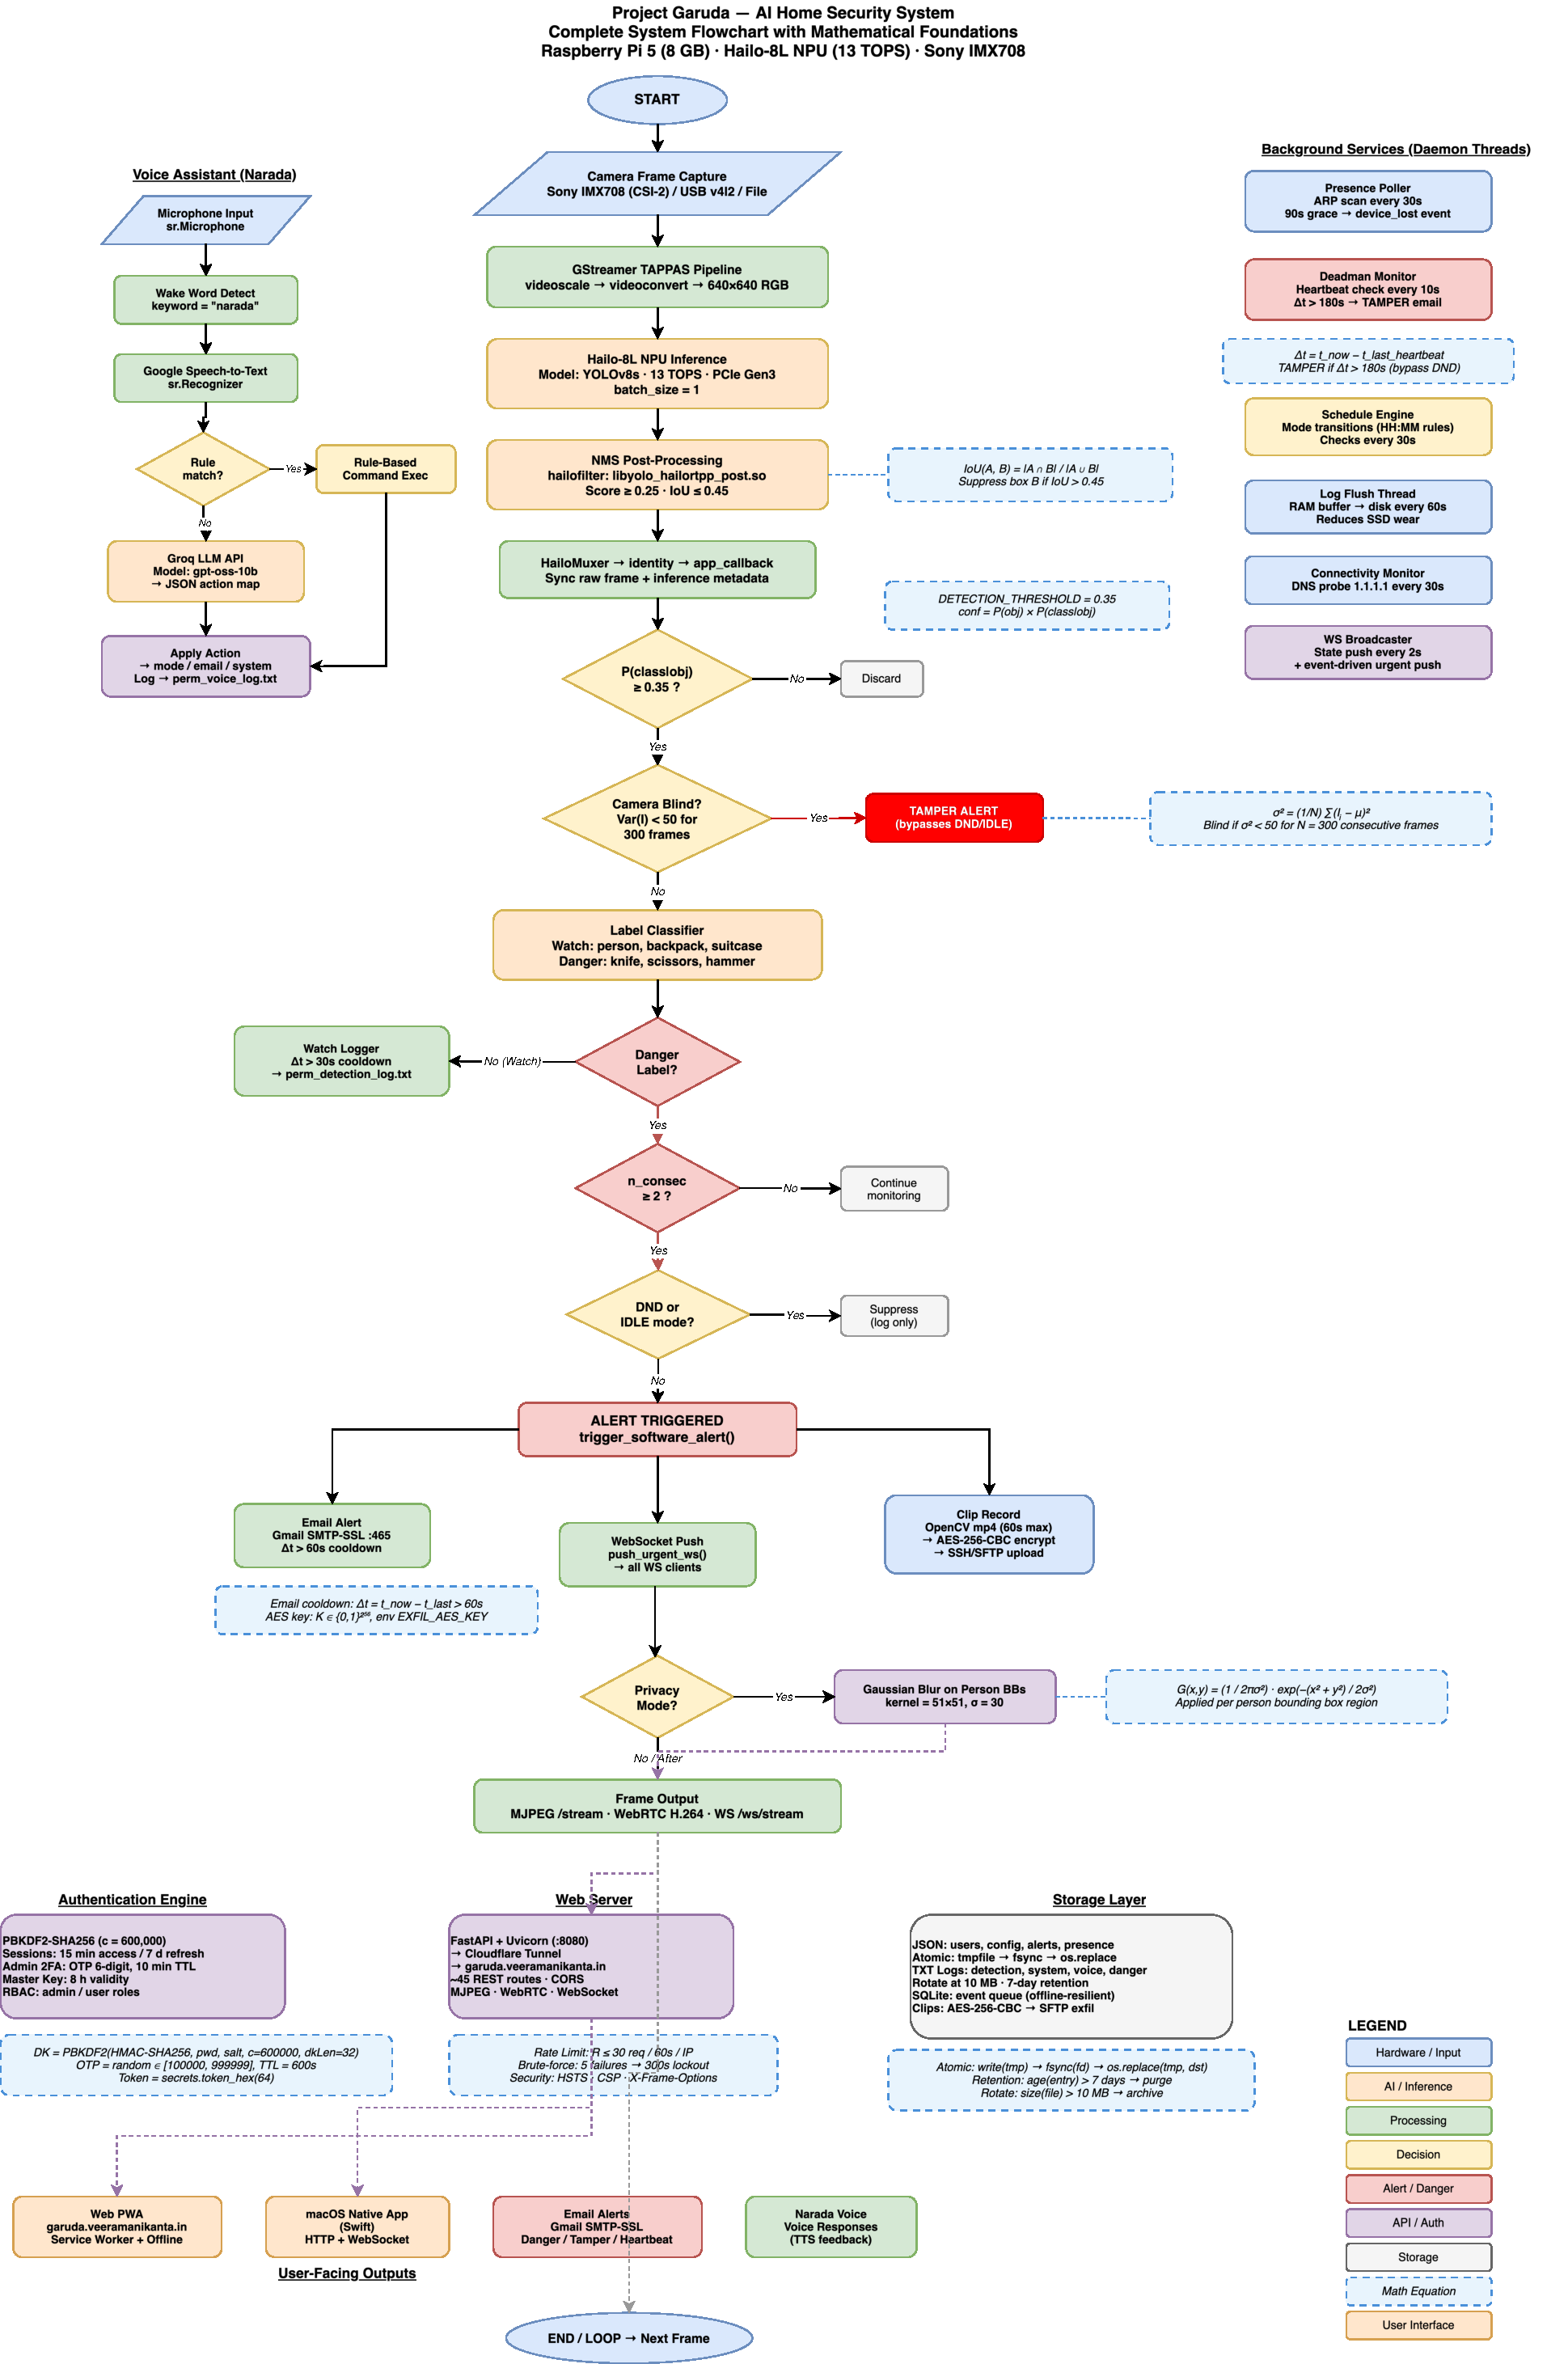
\includegraphics[width=0.92\textwidth,height=0.85\textheight,keepaspectratio]{garuda_system_flowchart.drawio.pdf}
\caption{Project Garuda system flowchart. Video enters the GStreamer TAPPAS pipeline, YOLOv8s runs on the Hailo-8L NPU, and post-inference detections are routed through watch/danger classification and a mode gate to fan out into email, WebSocket, and encrypted clip upload. Parallel subsystems---voice assistant, presence monitor, deadman watchdog, mode scheduler, authentication, and the Cloudflare-tunnelled web server---execute concurrently and feed the multi-tier logging engine.}
\label{fig:system_flowchart}
\end{figure*}

The overall block diagram in Fig.~\ref{fig:block_diagram} organises the system into three horizontal layers. The inference pipeline layer at the top carries video from the camera through the GStreamer TAPPAS pipeline into the Hailo-8L NPU, which runs YOLOv8s object detection and classifies detections as watch targets (\textit{Person}) or danger objects (\textit{Knife}, \textit{Scissors}, \textit{Hammer}). The response and control layer in the middle contains the alert engine, the voice assistant, the mode controller, and the presence monitor; these components are driven by detection events and collectively decide which actions to take based on the current operating mode. The web server and persistence layer at the bottom handles all external communication---FastAPI with Cloudflare tunnel, PBKDF2-based auth, the 180-second deadman watchdog, and the multi-tier logging engine---and every engine in the layers above writes events into this layer for storage and client delivery.

\begin{figure*}[!t]
\centering
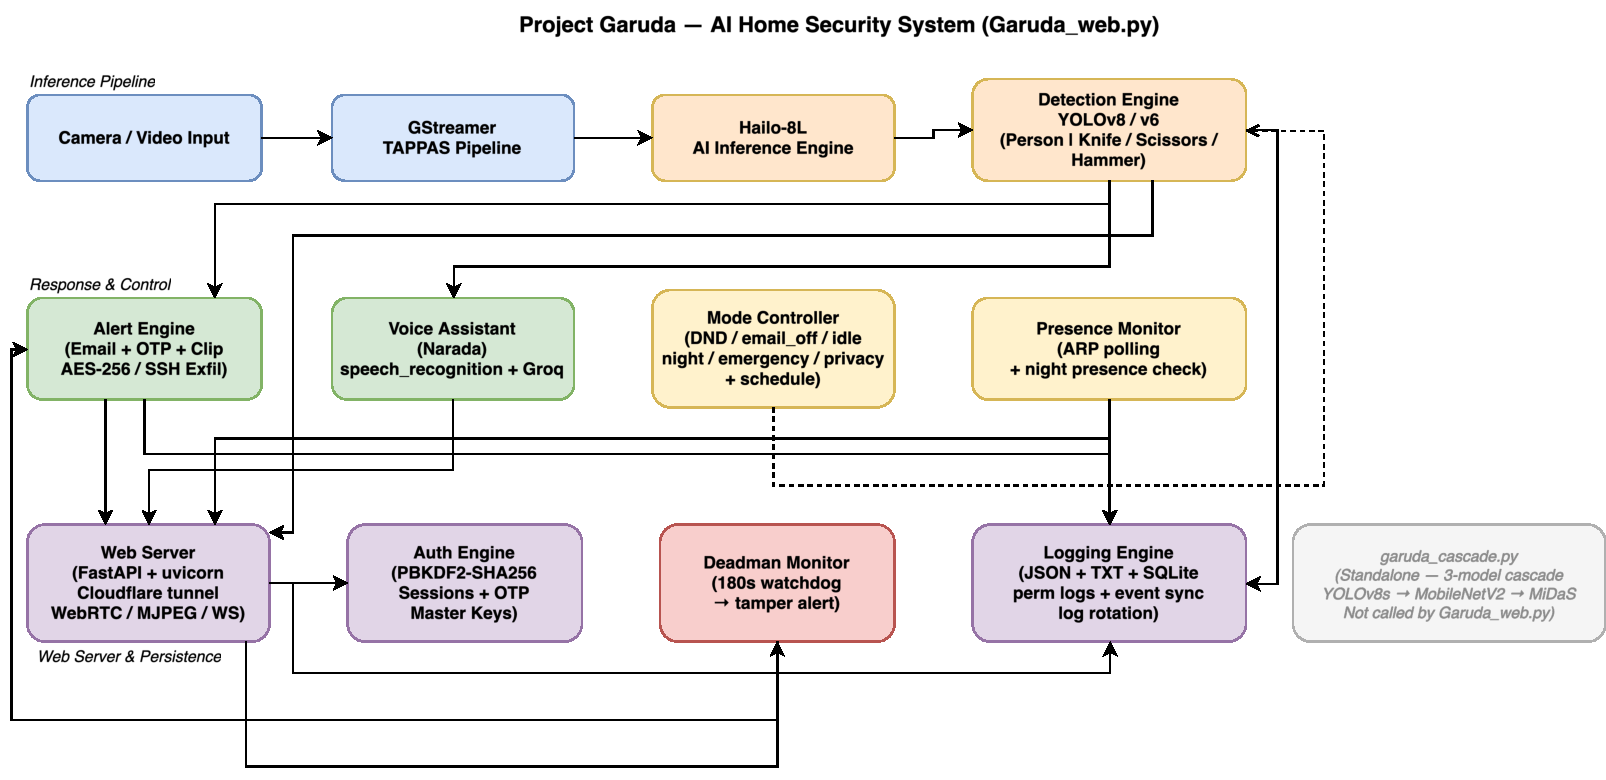
\includegraphics[width=0.9\textwidth,keepaspectratio]{garuda_block_diagram.drawio-3.pdf}
\caption{Three-layer block diagram. Top: inference pipeline (camera $\to$ GStreamer $\to$ Hailo-8L $\to$ detection classes). Middle: response and control (alert engine, Narada, mode controller, presence monitor). Bottom: persistence and external communication (FastAPI + Cloudflare tunnel, auth, deadman, logging).}
\label{fig:block_diagram}
\end{figure*}

\section{Specifications}
\label{sec:specs}
This section consolidates the hardware, software, model, and dataset specifications of the deployed system so that the results reported in Section~\ref{sec:results} can be reproduced on comparable hardware.

\subsection{Hardware}
Table~\ref{tab:hw_specs} lists the host board, accelerator, camera, and peripheral interfaces used for every reported measurement.

\begin{table}[!t]
\caption{\textbf{Hardware Specification}}
\label{tab:hw_specs}
\setlength{\tabcolsep}{3pt}
\centering
\begin{tabular}{|l|l|}
\hline
\textbf{Component} & \textbf{Specification} \\
\hline
Host board & Raspberry Pi 5 (BCM2712) \\
CPU & Quad-core Arm Cortex-A76 @ 2.4~GHz \\
RAM & 8~GB LPDDR4X-4267 \\
Storage & microSD / external USB-3 SSD \\
Neural accelerator & Hailo-8L AI HAT+ (13~TOPS, INT8) \\
NPU interface & PCIe Gen3 $\times$1 (M.2 M-key) \\
Device node & \texttt{/dev/hailo0} \\
Primary camera & Raspberry Pi Camera Module v3 (Sony IMX708) \\
Camera interface & CSI-2 MIPI (libcamera) \\
Secondary camera & USB webcam via V4L2 (\texttt{/dev/video0}) \\
Networking & Gigabit Ethernet + 802.11ac Wi-Fi \\
Power supply & 5~V / 5~A USB-C (official PSU) \\
Estimated BOM & US\$450--500 \\
\hline
\end{tabular}
\end{table}

\subsection{Software Stack}
The software stack is summarised in Table~\ref{tab:sw_specs}. The Hailo driver is installed as a DKMS module so that kernel upgrades do not break the PCIe interface, and all Python services run under a single virtual environment that is activated by the \texttt{setup\_env.sh} script.

\begin{table}[!t]
\caption{\textbf{Software Stack Specification}}
\label{tab:sw_specs}
\setlength{\tabcolsep}{3pt}
\centering
\begin{tabular}{|l|l|}
\hline
\textbf{Layer} & \textbf{Version / Package} \\
\hline
Operating system & Raspberry Pi OS (64-bit, Debian 12) \\
Kernel & Linux 6.12.x \\
Hailo driver & \texttt{hailo\_pci} 4.20.0 (DKMS) \\
Hailo runtime & HailoRT 4.20.0 \\
Hailo compiler & Hailo Dataflow Compiler v3.33.1 \\
TAPPAS framework & 3.28.x / 3.31.0 \\
GStreamer & 1.22 \\
Python & 3.11 \\
Web framework & FastAPI + Uvicorn \\
ASGI media & aiortc (WebRTC), \texttt{python-multipart} \\
Speech & \texttt{SpeechRecognition}, \texttt{PyAudio} \\
LLM backend & Groq API (\texttt{gpt-oss-120b}) \\
Auth primitives & \texttt{hashlib.pbkdf2\_hmac}, \texttt{secrets} \\
Crypto & AES-256-CBC (\texttt{cryptography}) \\
Remote exfiltration & \texttt{paramiko} (SSH) \\
Event database & SQLite 3.40 \\
Public ingress & Cloudflare Tunnel (\texttt{cloudflared}) \\
\hline
\end{tabular}
\end{table}

\subsection{Models}
Three neural networks are deployed. The primary detector is a YOLOv8s model fine-tuned on a custom four-class dataset and post-training-quantised to INT8 for the Hailo-8L. The classifier is a MobileNetV2 head that runs on cropped person regions, and the depth estimator is MiDaS Small for monocular anti-spoof verification in night mode. Table~\ref{tab:model_specs} summarises the three.

\begin{table}[!t]
\caption{\textbf{Model Specification}}
\label{tab:model_specs}
\setlength{\tabcolsep}{3pt}
\centering
\begin{tabular}{|l|l|}
\hline
\textbf{Attribute} & \textbf{Value} \\
\hline
Detector architecture & YOLOv8s \\
Detector classes & Hammer, Knife, Person, Scissors \\
Detector input size & $640\times640$ (letterbox) \\
Detector quantisation & INT8 PTQ (Hailo DFC v3.33.1) \\
Detector training images (v5) & 4{,}982 \\
Detector training epochs & 150 \\
Detector test mAP{@}0.5 & 0.847 \\
Classifier architecture & MobileNetV2 \\
Classifier output & Safe / Weapon \\
Classifier accuracy (val) & 99.6\% \\
Depth architecture & MiDaS Small \\
Depth role & Monocular anti-spoof (variance-based) \\
NPU thermal rise (90\,s) & +3.8$^\circ$C \\
End-to-end detection latency & $\sim$22~ms \\
\hline
\end{tabular}
\end{table}

\subsection{Dataset (v5)}
The deployed detector is trained on v5, a four-class dataset built by merging a Roboflow seed with OpenImages v7 samples. Table~\ref{tab:dataset} lists the dataset geometry.

\begin{table}[!t]
\caption{\textbf{v5 Dataset Geometry}}
\label{tab:dataset}
\setlength{\tabcolsep}{3pt}
\centering
\begin{tabular}{|l|l|}
\hline
\textbf{Property} & \textbf{Value} \\
\hline
Image format & JPEG (100\%) \\
Width (min / mean / max) & 436 / 826.1 / 4608~px \\
Height (min / mean / max) & 303 / 722.4 / 3456~px \\
Unique resolutions & 439 \\
Most common resolution & 640$\times$640 (2{,}187 images, 43.9\%) \\
File size (median / p95) & 148.8~KB / 621.2~KB \\
Total dataset size & 1.32~GB \\
Train / Val / Test images & 4{,}982 / 1{,}070 / 174 \\
Total images & 6{,}226 \\
Annotated instances & 16{,}335 \\
\hline
\end{tabular}
\end{table}

\section{Results}
\label{sec:results}
The deployed system is evaluated on two axes: \textit{model quality} on a held-out 174-image / 351-instance test set, and \textit{runtime performance} on the Hailo-8L under the deployed GStreamer pipeline. The evaluation covers training convergence, validation and test mAP, per-class precision/recall/mAP, confusion structure, precision-recall and F1-confidence behaviour, the effect of dataset size on generalisation, the validation-to-test gap, dataset distribution, and hardware throughput.

\subsection{Training Loss Convergence}
All three YOLOv8 loss components---box, classification, and distribution-focus---decrease monotonically over the full 150 training epochs, with box loss dropping from 1.65 to 0.74 and classification loss from 2.80 to 0.49. The close tracking between the training and validation curves confirms that the model generalises well and is not overfitting to the training distribution. The training dynamics are shown in Fig.~\ref{fig:training_losses}.

\begin{figure}[!t]
\centering

\includegraphics[width=\columnwidth]{fig1_training_losses.pdf}
\caption{Training loss convergence over 150 epochs: box, classification, and distribution-focus losses drop monotonically with no divergence between train and validation curves.}
\label{fig:training_losses}
\end{figure}

\subsection{Validation mAP and Precision/Recall}
mAP{@}0.5 rises sharply in the first 30 epochs and then plateaus near 0.81 by epoch 100, with mAP\text{@}0.5{:}0.95 following at $\sim$0.62. Precision and recall converge near 0.87 and 0.80 respectively, indicating a well-balanced detector with no strong bias toward false positives or false negatives. These curves are plotted in Fig.~\ref{fig:training_metrics}.

\begin{figure}[!t]
\centering

\includegraphics[width=\columnwidth]{fig2_training_metrics.pdf}
\caption{Validation mAP{@}0.5, mAP\text{@}0.5{:}0.95, precision, and recall versus epoch.}
\label{fig:training_metrics}
\end{figure}

\subsection{Three-Model Performance Comparison}
The default COCO-pretrained YOLOv8s scores near zero on all four metrics because its 80-class label scheme does not align with the 4-class task, confirming that out-of-the-box weights are completely unusable for this domain. Fine-tuned v1 (359 training images) recovers to a test mAP{@}0.5 of 0.465, and the final fine-tuned v5 (4{,}982 training images, 150 epochs) achieves a test mAP{@}0.5 of 0.847---an 82\% improvement over v1 and a 12\% gain over v2. This is visualised in Fig.~\ref{fig:model_comparison}.

\begin{figure}[!t]
\centering

\includegraphics[width=\columnwidth]{fig3_model_comparison.pdf}
\caption{Three-model comparison on the held-out test set: default COCO YOLOv8s versus fine-tuned v1 versus final v5.}
\label{fig:model_comparison}
\end{figure}

\subsection{Per-Class mAP{@}0.5 Progression}
The largest individual gain from v1 to v5 is achieved by the \textit{Knife} class, which improves by $+0.66$~mAP{@}0.5 because the Roboflow seed dataset contained very few diverse knife images. \textit{Scissors} achieves the highest absolute mAP{@}0.5 of 0.967 in v5, while \textit{Person} remains the most challenging class at 0.647, reflecting high intra-class visual variability across poses, occlusions, and backgrounds. All four classes improve monotonically from v1 through v2 to v5, as shown in Fig.~\ref{fig:per_class_map} and Table~\ref{tab:v1_v5}.

\begin{figure}[!t]
\centering

\includegraphics[width=\columnwidth]{fig4_per_class_map50.pdf}
\caption{Per-class mAP{@}0.5 at v1, v2, and v5. All four classes improve monotonically with dataset scale.}
\label{fig:per_class_map}
\end{figure}

\begin{table*}[!t]
\caption{\textbf{Per-Class Recall and mAP{@}0.5: v1 vs v5 (Deployed)}}
\label{tab:v1_v5}
\centering
\begin{tabular}{|l|c|c|c|c|c|c|}
\hline
\textbf{Class} & \textbf{v1 Recall} & \textbf{v5 Recall} & \textbf{Recall Gain} & \textbf{v1 mAP{@}0.5} & \textbf{v5 mAP{@}0.5} & \textbf{mAP{@}0.5 Gain} \\
\hline
Hammer   & 0.663 & 0.848 & +27.9\% & 0.632 & 0.889 & +40.7\% \\
Knife    & 0.267 & 0.817 & +206\%  & 0.229 & 0.886 & +287\% \\
Person   & 0.197 & 0.609 & +209\%  & 0.240 & 0.647 & +170\% \\
Scissors & 0.761 & 0.929 & +22.1\% & 0.760 & 0.967 & +27.2\% \\
\hline
\textbf{All} & \textbf{0.472} & \textbf{0.801} & \textbf{+69.7\%} & \textbf{0.465} & \textbf{0.847} & \textbf{+82.2\%} \\
\hline
\end{tabular}
\end{table*}

\subsection{Full Per-Class Metrics at v5}
On the held-out test set, \textit{Hammer}, \textit{Knife}, and \textit{Scissors} all achieve balanced performance with precision and recall above 0.82, while \textit{Person} is the weakest class with precision 0.701 and recall 0.609---a direct consequence of its higher intra-class visual variability. \textit{Scissors} achieves an exceptional mAP{@}0.5 of 0.967 and mAP\text{@}0.5{:}0.95 of 0.828, making it the best-detected class overall. The full per-class breakdown is plotted in Fig.~\ref{fig:perclass_full} and enumerated in Table~\ref{tab:perclass_tpfn}.

\begin{figure}[!t]
\centering

\includegraphics[width=\columnwidth]{fig5_perclass_full_metrics.pdf}
\caption{Full per-class metrics (precision, recall, mAP{@}0.5, mAP\text{@}0.5{:}0.95) for the deployed v5 model.}
\label{fig:perclass_full}
\end{figure}

\begin{table}[!t]
\caption{\textbf{Per-Class TP/FN and Detection Recall (v5 Test Set)}}
\label{tab:perclass_tpfn}
\setlength{\tabcolsep}{4pt}
\centering
\begin{tabular}{|l|c|c|c|}
\hline
\textbf{Class} & \textbf{TP} & \textbf{FN} & \textbf{Recall} \\
\hline
Hammer   & \texttildelow39   & \texttildelow7   & 0.848 \\
Knife    & \texttildelow130  & \texttildelow29  & 0.817 \\
Person   & \texttildelow807  & \texttildelow517 & 0.609 \\
Scissors & \texttildelow118  & \texttildelow9   & 0.929 \\
\hline
\textbf{Overall} & \textbf{\texttildelow1,094} & \textbf{\texttildelow562} & \textbf{0.801} \\
\hline
\end{tabular}
\end{table}

\subsection{Normalised Confusion Matrix}
The normalised confusion matrix in Fig.~\ref{fig:confusion} is diagonally dominant, with correct-class recall values of 0.85, 0.82, 0.61, and 0.93 for \textit{Hammer}, \textit{Knife}, \textit{Person}, and \textit{Scissors} respectively. Inter-class confusion is low ($\leq 0.03$ per off-diagonal cell), meaning the bulk of errors are outright misses (background false negatives) rather than misclassifications between the four target classes---an important property for a security system where a misclassified weapon is more dangerous than a missed one because it still triggers an alert.

\begin{figure}[!t]
\centering

\includegraphics[width=\columnwidth]{fig6_confusion_matrix.pdf}
\caption{Normalised confusion matrix on the v5 held-out test set. Diagonal dominance confirms strong per-class discrimination with inter-class confusion $\leq 0.03$.}
\label{fig:confusion}
\end{figure}

\subsection{Precision-Recall Curves}
\textit{Scissors} has the highest area under the precision-recall curve (AP = 0.967) and maintains high precision well past a recall of 0.90, while \textit{Person} shows the steepest precision drop-off at lower recall thresholds, consistent with its higher intra-class variability. \textit{Knife} and \textit{Hammer} both exhibit smooth, well-separated curves with APs of 0.886 and 0.889 respectively, demonstrating reliable detection across a wide confidence operating range. The full set of PR curves is shown in Fig.~\ref{fig:pr_curves}.

\begin{figure}[!t]
\centering

\includegraphics[width=\columnwidth]{fig7_pr_curves.pdf}
\caption{Per-class precision-recall curves for the deployed v5 detector on the held-out test set.}
\label{fig:pr_curves}
\end{figure}

\subsection{Dataset Class Distribution}
\textit{Person} is the most represented class with 2{,}100 training instances, while \textit{Hammer} is the scarcest at 480, reflecting the natural frequency imbalance in the source datasets. This imbalance partially explains \textit{Person}'s lower precision (0.701)---abundant training examples introduce more background diversity and harder negatives---while the full 4{,}982-image training set allows v5 to substantially outperform earlier checkpoints on every class. The class distribution across the train/val/test splits is plotted in Fig.~\ref{fig:dataset_dist}, and the dataset growth across versions is summarised in Table~\ref{tab:dataset_versions}.

\begin{figure}[!t]
\centering

\includegraphics[width=\columnwidth]{fig8_dataset_distribution.pdf}
\caption{v5 dataset class distribution across train, validation, and test splits.}
\label{fig:dataset_dist}
\end{figure}

\begin{table}[!t]
\caption{\textbf{Dataset Versions: Growth and Test mAP}}
\label{tab:dataset_versions}
\setlength{\tabcolsep}{2pt}
\centering\footnotesize
\begin{tabular}{|l|c|c|c|c|p{3.2cm}|}
\hline
\textbf{Ver.} & \textbf{Train} & \textbf{Total} & \textbf{Inst.} & \textbf{mAP50} & \textbf{Primary change} \\
\hline
v1 & 359   & 512   & $\sim$1{,}200  & 0.465 & Roboflow seed only \\
v2 & 1{,}383 & 1{,}730 & $\sim$4{,}000  & 0.754 & + OpenImages v7 (1{,}219 imgs) \\
v5 & 4{,}982 & 6{,}226 & 16{,}335       & 0.847 & + OI per-class (2{,}276 imgs) \\
\hline
\end{tabular}
\end{table}

\subsection{MobileNetV2 Classifier Split}
The MobileNetV2 \textit{Safe}/\textit{Weapon} classifier is trained on cropped regions harvested from the detection pipeline. The split is summarised in Table~\ref{tab:mobilenet}.

\begin{table}[!t]
\caption{\textbf{MobileNetV2 Classifier Dataset}}
\label{tab:mobilenet}
\setlength{\tabcolsep}{4pt}
\centering
\begin{tabular}{|l|c|c|c|}
\hline
\textbf{Split} & \textbf{Safe crops} & \textbf{Weapon crops} & \textbf{Total} \\
\hline
Train & 1{,}200 & 1{,}660 & 2{,}860 \\
Val   & 200     & 24      & 224 \\
\hline
\end{tabular}
\end{table}

\subsection{Hardware Inference Performance}
The custom \texttt{best\_v5.hef} model achieves 52.2~FPS at 18.4~ms NPU latency on the Hailo-8L, comfortably exceeding the real-time requirement ($\geq 25$~FPS) for security surveillance. This compares favourably against the reference Hailo-distributed YOLOv8s (13.2~ms / 58.2~FPS); the modest 5~ms latency increase is attributable to the custom NMS post-processing baked into the HEF. Even with the small FPS delta, we remain well above the 30~FPS operating threshold and under the 50~ms latency ceiling, so the difference has no practical effect at runtime. The reference models run marginally faster because they were pre-optimised by the Hailo team for the exact fixed post-processing chain shipped in HailoRT. Fig.~\ref{fig:hw_perf} visualises the latency/throughput comparison. Compared with prior edge-deployed detectors, our 52.2~FPS exceeds the 36.7~FPS reported by Xu~\emph{et~al.}~\cite{b1} for FL-YOLO on an NVIDIA Jetson TX1 and far surpasses the 15~FPS of Al~Amin~\emph{et~al.}'s FPGA implementation~\cite{b5}, while operating at a comparable mAP{@}0.5 of 0.847 on our domain-specific four-class task.

\begin{figure}[!t]
\centering

\includegraphics[width=\columnwidth]{fig9_hardware_performance.pdf}
\caption{Hardware inference performance on the Hailo-8L: custom v5 HEF (52.2~FPS, 18.4~ms) versus the Hailo-provided YOLOv8s reference (58.2~FPS, 13.2~ms).}
\label{fig:hw_perf}
\end{figure}

\subsection{F1-Confidence Threshold Curves}
All four classes reach their peak F1 score in the confidence range 0.25--0.27, which aligns with YOLO's default threshold of 0.25 and confirms that no manual threshold tuning is required for deployment. \textit{Scissors} achieves the highest peak F1 (0.690), while \textit{Person} is lowest (0.473), consistent with its lower recall; operating slightly below the peak threshold for \textit{Person} can recover additional true positives at a modest false-positive cost. The F1-confidence sweep is shown in Fig.~\ref{fig:f1_conf}.

\begin{figure}[!t]
\centering

\includegraphics[width=\columnwidth]{fig10_f1_confidence.pdf}
\caption{Per-class F1 score versus confidence threshold; peak F1 sits in the 0.25--0.27 band for all four classes.}
\label{fig:f1_conf}
\end{figure}

\subsection{Effect of Training Dataset Size}
Fine-tuned v1 (359 images) converges quickly to a high validation mAP of $\sim$0.88, but its held-out test mAP is only 0.465---exposing severe overfitting to the Roboflow dataset's visual style. Fine-tuned v2 (1{,}383 images) narrows the gap substantially (val 0.735, test 0.754), and the final v5 (4{,}982 images, 150 epochs) achieves both strong validation (0.817) and the best test mAP (0.847). This confirms that dataset scale and diversity---not architectural changes---are the dominant factors for real-world generalisation on this task. The effect is plotted in Fig.~\ref{fig:v1v2}.

\begin{figure}[!t]
\centering

\includegraphics[width=\columnwidth]{fig11_v1_vs_v2_training.pdf}
\caption{Validation mAP{@}0.5 progression versus training dataset size (v1, v2, v5).}
\label{fig:v1v2}
\end{figure}

\subsection{Validation-to-Test Generalisation Gap}
Fine-tuned v1 exhibits a 0.414-point gap between its best validation mAP (0.879) and its held-out test mAP (0.465)---a clear sign of distribution overfit to the single-source Roboflow dataset. Fine-tuned v2 slightly reverses this gap ($+0.019$, test marginally beats val), and the final v5 achieves a positive generalisation gap ($+0.030$: test 0.847 $>$ val 0.817), confirming that the expanded 4{,}982-image dataset produces a model that generalises robustly to genuinely unseen real-world imagery. Fig.~\ref{fig:overfit} visualises this progression.

\begin{figure}[!t]
\centering

\includegraphics[width=\columnwidth]{fig12_overfitting_gap.pdf}
\caption{Validation-to-test mAP{@}0.5 gap across v1, v2, and v5. The final v5 achieves positive generalisation (test $>$ val).}
\label{fig:overfit}
\end{figure}


\section{Conclusion}
\label{sec:conclusion}
Project Garuda demonstrates that a self-hosted, privacy-first, cloud-independent AI home security system can be built from consumer hardware for under US\$500 without compromising on real-time performance or modern security primitives. The core engineering claim of the system is that a Raspberry Pi 5 paired with a Hailo-8L AI HAT+ can host the full inference stack---a custom-fine-tuned YOLOv8s detector for four threat-relevant classes, a MobileNetV2 classifier for \textit{Safe}/\textit{Weapon} verification, and a MiDaS Small depth estimator for monocular anti-spoof---at 52.22~FPS and 18.38~ms NPU latency, well inside the real-time envelope for continuous surveillance, while leaving the CPU free to run the FastAPI web server, the Narada voice assistant, the presence monitor, the deadman watchdog, and the logging engine concurrently.

On the model side, the progression from a 359-image v1 ($\text{mAP}_{50}=0.465$) to the 4{,}982-image v5 ($\text{mAP}_{50}=0.847$) with a $+0.030$ positive validation-to-test generalisation gap confirms that dataset scale and diversity---not architectural changes---are the dominant lever for robust real-world performance, and that the COCO baseline of 0.0002~mAP on this 4-class task is essentially random, reinforcing the need for targeted fine-tuning on security-relevant classes. The low off-diagonal values in the confusion matrix ($\leq 0.03$) and the alignment of the peak F1 confidence with YOLO's default 0.25 threshold mean the model ships without requiring any post-deployment threshold tuning.

On the systems side, the multi-engine architecture---alert fan-out with 60-second SMTP cooldown, WebSocket push, AES-256-CBC clip encryption, and SSH exfiltration; PBKDF2-SHA256 with 600{,}000 iterations and OTP 2FA; the 180-second deadman watchdog; six lock-guarded and scheduler-driven operating modes; ARP-based LAN presence; and the SQLite-backed offline event sync---closes the gap identified in the introduction between DIY motion-only setups and cloud-dependent professional systems. Every event reaches the dashboard in real time over WebSocket or WebRTC, and every event is also persisted to the multi-tier logger for offline catch-up, giving browser clients a coherent view of the system state even after arbitrary network outages.

The broader implication is that edge AI is no longer a compromise. With the right accelerator, the right post-training quantisation flow, and a disciplined software architecture, a device the size of a paperback can deliver detection quality, response latency, and security properties that previously required a cloud subscription and a server rack. Future extensions worth pursuing include expanding the class vocabulary beyond the four threat-relevant labels, exploring temporal models for activity recognition on top of the detector, integrating on-device TTS so that Narada remains functional when the public network is unavailable, and replacing the current static MiDaS variance threshold with a learned liveness head that is co-trained with the detector.



\begin{thebibliography}{00}

\bibitem{b1} Z.~Xu, J.~Li, and M.~Zhang, ``A surveillance video real-time analysis system based on edge-cloud and FL-YOLO cooperation in coal mine,'' \emph{IEEE Access}, vol.~9, pp.~161~498--161~512, 2021.

\bibitem{b2} J.~Redmon, S.~Divvala, R.~Girshick, and A.~Farhadi, ``You only look once: Unified, real-time object detection,'' in \emph{Proc. IEEE Conf. Comput. Vis. Pattern Recognit. (CVPR)}, Las Vegas, NV, USA, 2016, pp.~779--788.

\bibitem{b3} Hailo Technologies Ltd., ``Hailo-8L M.2 AI acceleration module datasheet,'' 2024. [Online]. Available: https://hailo.ai/products/ai-accelerators/hailo-8l-ai-accel-for-ai-light-applications/

\bibitem{b4} G.~Bueno \emph{et~al.}, ``Real-time edge computing vs.\ GPU-accelerated pipelines for low-cost microscopy applications,'' \emph{Electronics}, vol.~14, no.~6, Art.~no.~930, 2025.

\bibitem{b5} R.~Al~Amin, M.~Hasan, V.~Wiese, and R.~Obermaisser, ``FPGA-based real-time object detection and classification system using YOLO for edge computing,'' \emph{IEEE Access}, vol.~12, pp.~61~080--61~093, 2024.

\bibitem{b6} C.~Dong, C.~Pang, Z.~Li, X.~Zeng, and X.~Hu, ``PG-YOLO: A novel lightweight object detection method for edge devices in industrial Internet of Things,'' \emph{IEEE Access}, vol.~10, pp.~40~177--40~186, 2022.

\bibitem{b7} M.-A.~Chung \emph{et~al.}, ``YOLO-LSD: A lightweight object detection model for small targets at long distances to secure pedestrian safety,'' \emph{IEEE Access}, vol.~13, pp.~14~520--14~534, 2025.

\bibitem{b8} F.~Cheng, ``Accurate detection of solar panel defects using RMN-YOLO with multi-scale edge and attention enhancements,'' \emph{IEEE Access}, vol.~13, pp.~25~632--25~645, 2025.

\bibitem{b9} G.~Jocher, A.~Chaurasia, and J.~Qiu, ``Ultralytics YOLOv8,'' 2023. [Online]. Available: https://github.com/ultralytics/ultralytics

\bibitem{b10} Hailo Technologies Ltd., ``TAPPAS --- Hailo's AI application development framework,'' 2024. [Online]. Available: https://github.com/hailo-ai/tappas

\bibitem{b11} Raspberry Pi Ltd., ``Raspberry Pi 5 product brief,'' 2023. [Online]. Available: https://www.raspberrypi.com/products/raspberry-pi-5/

\bibitem{b12} S.~Ram\'{i}rez, ``FastAPI --- Modern, fast web framework for building APIs with Python,'' 2019. [Online]. Available: https://fastapi.tiangolo.com

\bibitem{b13} GStreamer Team, ``GStreamer: Open source multimedia framework,'' 2024. [Online]. Available: https://gstreamer.freedesktop.org

\bibitem{b14} R.~Ranftl, K.~Lasinger, D.~Hafner, K.~Schindler, and V.~Koltun, ``Towards robust monocular depth estimation: Mixing datasets for zero-shot cross-dataset transfer,'' \emph{IEEE Trans. Pattern Anal. Mach. Intell.}, vol.~44, no.~3, pp.~1623--1637, Mar. 2022.

\bibitem{b15} M.~Sandler, A.~Howard, M.~Zhu, A.~Zhmoginov, and L.-C.~Chen, ``MobileNetV2: Inverted residuals and linear bottlenecks,'' in \emph{Proc. IEEE Conf. Comput. Vis. Pattern Recognit. (CVPR)}, Salt Lake City, UT, USA, 2018, pp.~4510--4520.

\bibitem{b16} B.~Kaliski, ``PKCS \#5: Password-based cryptography specification version 2.0,'' RFC 2898, Internet Eng. Task Force, Sep. 2000.

\bibitem{b17} Cloudflare, Inc., ``Cloudflare Tunnel documentation,'' 2024. [Online]. Available: https://developers.cloudflare.com/cloudflare-one/connections/connect-networks/

\end{thebibliography}

\EOD

\end{document}
